\documentclass[11pt,a4paper]{article}
\usepackage[margin=24mm,headheight=14pt]{geometry}
\usepackage[T1]{fontenc}
\usepackage{lmodern}
\usepackage{amsmath,amssymb,mathtools}
\usepackage{booktabs,longtable,array}
\usepackage{microtype}
\usepackage{xcolor}
\usepackage{enumitem}
\usepackage{fancyhdr}
\usepackage{pgfplots}
\pgfplotsset{compat=1.18}
\usepackage[hidelinks,breaklinks]{hyperref}
\definecolor{atlasblue}{RGB}{24,65,98}
\definecolor{atlasorange}{RGB}{183,91,31}
\hypersetup{pdftitle={CANSAT: mathematical derivations and verification},pdfauthor={CANSAT project}}
\pagestyle{fancy}
\fancyhf{}
\fancyhead[L]{\small CANSAT mathematics}
\fancyhead[R]{\small Analysis: 30 September 2026; platform note: 13 October 2026}
\fancyfoot[C]{\thepage}
\setlength{\parindent}{0pt}
\setlength{\parskip}{5pt plus 1pt}
\setlength{\emergencystretch}{2em}
\setlist[itemize]{topsep=3pt,itemsep=2pt}
\setlist[enumerate]{topsep=3pt,itemsep=2pt}
\allowdisplaybreaks[2]
\numberwithin{equation}{section}
\setcounter{tocdepth}{1}
\newcommand{\R}{\mathbb R}
\newcommand{\E}{\operatorname E}
\newcommand{\Var}{\operatorname{Var}}
\newcommand{\Cov}{\operatorname{Cov}}
\newcommand{\tr}{\operatorname{tr}}
\newcommand{\diag}{\operatorname{diag}}
\begin{document}
\begin{titlepage}
\vspace*{16mm}
{\color{atlasblue}\Huge\bfseries CANSAT\\[4mm] Mathematical derivations\\[4mm] and verification\par}
\vspace{9mm}
{\Large A readable reference for terrain-relative navigation,\\wind retrieval and landing prediction\par}
\vspace{8mm}
{\large 30 September 2026\par}
\vspace{14mm}
\textbf{Purpose.} Derive the mathematics required by the project's secondary-mission proposal, explain what each equation means, state the conditions under which it is valid, and verify the results with independent numerical identities and synthetic experiments.

\textbf{Basis.} The derivations and numerical examples originated from the local proposal dated 27 September 2026, including its mathematical index and Appendices A--L. Their stated model inputs and retained results remain historical and illustrative; they are not silently recalculated for the current hardware. The current component baseline is the Raspberry Pi Zero 2 W and STM32F405RGT6, BMI088 IMU, MS5611 barometer, GA10K3MCD1 probe with ADS1115/OPA333/150 k$\Omega$ interface, IMX296 global-shutter camera with Edmund 34-711/53-675 optics, 2S battery, E22 radio and MAX-M10S GNSS. The native image is 1456$\times$1088 pixels. The current compute target is 5 Hz, which has not been demonstrated on the Pi Zero 2 W. See the project \href{run:design_baseline.md}{design baseline} for the current configuration and source links. This workspace contains no flight calibration dataset or measured descent logs. The connected CANSAT 2027 reference folder was inspected; its available regulations PDF describes the 2025--2026 competition. It is historical context, not confirmation of 2026--2027 rules.

\textbf{Evidence levels.} An algebraic identity can be proved within a model. A simulation checks implementation and consequences of that model. Agreement with the physical CanSat requires measurements. This document keeps those three statements separate.

\textbf{Deliverable.} This source contains the entire document, including plotted coordinates. It needs no external figures, bibliography, or included source files. Supporting scripts retain reproducible checks and synthetic data in the project, but are not required to compile this document.
\vfill
{\small Design inputs are identified as assumptions; no synthetic value is presented as a measured flight result.}
\end{titlepage}
\tableofcontents
\clearpage

\section{How to read this document}
\label{sec:guide}
The mission has a connected chain of mathematics. A camera and inertial sensors estimate the probe's motion; a dynamic response model converts that motion to an atmospheric wind profile; a statistical wind model propagates the remaining drift to predict landing. Pressure and temperature provide density, height and stability. A wrong assumption early in this chain can produce convincing but biased results later.

Each section explains the model, derives its equations, and gives numerical or limiting-case checks. For a first reading, follow the physical dynamics, then the camera and filter, then turbulence, retrieval, and prediction. The supporting-engineering section supplies quantities needed to make the data collection possible. The final sections distinguish completed verification from the experiments still needed.

\subsection{Conventions and units}
\begin{center}
\begin{tabular}{p{0.21\linewidth}p{0.65\linewidth}}
\toprule
Symbol & Meaning and convention\\
\midrule
$z,h$ & Height above the stated terrain datum, upward positive (m).\\
$s,v_d$ & Distance descended (m) and positive downward speed (m/s).\\
$\boldsymbol u,\boldsymbol w$ & Probe velocity and atmospheric wind, respectively (m/s).\\
$g$ or $g_0$ & Positive gravitational acceleration, $9.80665$ m/s$^2$ in examples.\\
$g(r)$ & A \emph{different} object: dimensionless transverse correlation.\\
$L,L_p,L_O,\ell$ & Turbulence decay scale, suspension length, Obukhov length and horizontal lag length (m).\\
$R_{wb},R_{cb}$ & Body-to-world and body-to-camera rotations.\\
$\theta$ & Potential temperature in atmospheric sections; an explicitly vector-valued local rotation error in navigation.\\
$P,\Sigma,S$ & Covariances, with squared units of the variables concerned.\\
$\Delta t,\Delta s$ & Time and descended-distance sample intervals, both positive.\\
\bottomrule
\end{tabular}
\end{center}
Convert degrees to radians before using $h\delta\theta$ or angular-rate products. Use absolute temperature in kelvin and pressure in pascals except where a pressure ratio uses consistent units. Logarithms of lengths must be ratios to a stated reference length.

\subsection{Important corrections to the proposal}
The following are results of the mathematical audit; they do not silently replace a flight design decision.
\begin{enumerate}
\item The lag $\ell=v_d^2/g$ follows from isotropic vector drag, not from vertical canopy force balance alone. A measured lateral response coefficient is needed to justify it.
\item The stated shear example gives a horizontal offset of $23.8$ m over $100$ m of descent. A vertical-path approximation is conditional, rather than accurate to a few percent at every scale.
\item The warped turbulence coordinate must increase with descent. A positive time derivative is inconsistent with an upward-increasing definition.
\item A body-axis accelerometer can be blind to swing under an ideal suspension, but gyro angular acceleration cannot determine arbitrary static tilt or unknown forcing.
\item A temperature lapse does not determine Obukhov length. The bulk Richardson number is not the gradient stability theorem, and $0.25$ is not a universal turbulence cutoff.
\item Tilt and translation are separated by landmark geometry. Placing every landmark at the same off-axis radius is not, by itself, enough.
\item An RMS or protection-level claim must state its dimension, truth uncertainty, correlations and probability model. A three-standard-deviation one-axis rule is not a two-dimensional integrity rule.
\item RANSAC's $w=0.5$, two-point, $p=0.999$ example needs $25$ iterations after rounding up. Truncated least squares requires a proper lifted formulation before claiming an SDP certificate.
\item The greedy guarantee applies to normalised log-determinant improvement. It does not justify a scale-dependent multiplicative claim about raw log determinant.
\item Remaining drift and absolute landing position have different covariance behaviour. The latter has a monotonic conditioning theorem under a fixed linear Gaussian model.
\end{enumerate}

\subsection{Verification approach}
Analytic derivations are accompanied by checks that use a different route: direct projection against homography, finite differences against analytic Jacobians, numerical ODE integration against closed forms, Fourier quadrature against a rational spectrum, and batch Gaussian conditioning against Kalman/RTS inference. A successful test is evidence for the checked identity, not for every untested implementation detail.

Lean certificates are not included. The ordinary linear algebra, calculus and probability identities are stated with their hypotheses and verified by independent calculations. The remaining uncertainty concerns unmeasured physical parameters, field representativeness, algorithmic assumptions and finite data; a formal certificate for algebra would not resolve those issues.
\clearpage


\section{Descent, wind response and suspension physics}
\label{sec:physics}

This section verifies Appendix F and the physical inputs to the wind
retrieval. Equations are consequences of the stated models, not proof that
an unmeasured parachute obeys those models. Numerical examples use proposal
values as design inputs, not flight measurements. Take $z$ positive upwards,
$s=z(0)-z$ positive downwards, $v_d=\dot s>0$, and
$g=9.80665\,\mathrm{m\,s^{-2}}$ for the numerical checks. Horizontal vehicle
velocity is $\boldsymbol u$, and horizontal air velocity is $\boldsymbol w$.
The suspension length $L_p$, turbulence scale $L$, and Obukhov length $L_O$
are different quantities.

\subsection{Terminal descent and canopy sizing}

For a deployed, approximately steady canopy, negligible buoyancy, no
vertical wind, and effective vertical drag area $D_z=C_{D,z}A$, Newton's
law in the downward direction is
\begin{equation}
 m\dot v_d=mg-\tfrac12\rho D_z v_d^2.
\end{equation}
Setting $\dot v_d=0$ gives
\begin{equation}
 v_t=\sqrt{\frac{2mg}{\rho D_z}},\qquad
 D_z=\frac{2mg}{\rho v_t^2},\qquad
 \rho=\frac{p}{R_dT_v}.
\end{equation}
Here $p$ is in pascals, $T_v$ is virtual temperature in kelvin, and
$R_d$ is the dry-air specific gas constant. In dry air $T_v=T$; neglecting
humidity otherwise is an approximation. $m$ must be the total mass supported
by the aerodynamic system, with the convention for canopy mass stated.
For a circular reference area $A=\pi d^2/4$,
\begin{equation}
 d=\sqrt{\frac{8mg}{\pi\rho C_{D,z}v_t^2}}.
\end{equation}
The area convention used with a quoted coefficient must match the convention
in this formula. Neither a numerical $C_D$ nor a finished canopy diameter is
established by the proposal.

If $v_{\min}\leq v_t\leq v_{\max}$ is a specified design band, then
\begin{equation}
 \frac{2mg}{\rho v_{\max}^2}\leq D_z
 \leq\frac{2mg}{\rho v_{\min}^2}.
\end{equation}
For uncertain $m,\rho,D_z$, the slowest terminal speed occurs at smallest
$m$ and largest $\rho D_z$, and the fastest at the opposite corner of the
uncertainty set. First-order fractional sensitivity is
\begin{equation}
 \frac{\delta v_t}{v_t}
 =\frac12\left(\frac{\delta m}{m}-\frac{\delta\rho}{\rho}
 -\frac{\delta C_D}{C_D}-\frac{\delta A}{A}\right).
\end{equation}
This is a differential identity; root-sum-square uncertainty requires
uncorrelated errors or the appropriate covariance terms.

\subsection{Transient and variable descent speed}

For constant parameters and release from rest, separating variables gives
\begin{align}
 \int_0^{v_d/v_t}\frac{dq}{1-q^2}&=\frac{gt}{v_t},\\
 v_d(t)&=v_t\tanh(gt/v_t),\\
 s(t)&=\frac{v_t^2}{g}\ln\cosh(gt/v_t).
\end{align}
Thus a $300\,\mathrm m$ descent at a constant
$10.5\,\mathrm{m\,s^{-1}}$ takes $28.57\,\mathrm s$, whereas the ideal
fully deployed release-from-rest model gives
\begin{equation}
 t(H)=\frac{v_t}{g}\operatorname{arcosh}
       \left[\exp\left(\frac{gH}{v_t^2}\right)\right]
 \simeq29.31\,\mathrm s\quad(H=300\,\mathrm m).
\end{equation}
The latter assumes instantaneous deployment and is not an inflation model.
Linearization around $v_t$ gives
\begin{equation}
 \delta\dot v=-\frac{2g}{v_t}\delta v,
 \qquad \tau_z=\frac{v_t}{2g}.
\end{equation}
The vertical relaxation time is half the horizontal time in the isotropic
drag approximation derived below.

For variable density or drag, integrate the dynamical equation with
$\dot z=-v_d$ instead of imposing instantaneous terminal equilibrium.
If quasi-steady descent is justified, then
\begin{equation}
 t_{\rm remaining}=\int_0^h\frac{dz}{v_d(z)},\qquad
 \Delta\boldsymbol x=\int_0^h\frac{\boldsymbol u(z)}{v_d(z)}\,dz.
\end{equation}
Quasi-steady tracking requires the fractional equilibrium-speed change
over $\tau_z$ to be small. A vertical air velocity $w_z$, positive upwards,
changes the air-relative downward speed to $v_d+w_z$; ground-relative
descent speed cannot then be substituted indiscriminately in drag.
Perturbing the first integral yields
\begin{equation}
 \delta t=\frac{\delta h}{v_d(h)}
 -\int_0^h\frac{\delta v_d(z)}{v_d(z)^2}\,dz.
\end{equation}
Altitude and descent-model uncertainty therefore both enter touchdown time.

\subsection{Pressure altitude: the precise hypsometric equation}

Hydrostatic balance $dp/dz=-\rho g$ and the ideal gas relation give
\begin{equation}
 dz=-\frac{R_dT_v}{g}\,d\ln p.
\end{equation}
With approximately constant $g$ over the layer,
\begin{align}
 z_2-z_1&=\frac{R_d}{g}\int_{p_2}^{p_1}T_v(p)\,d\ln p\\
 &=\frac{R_d\overline T_v^{\ln p}}{g}\ln(p_1/p_2),\\
 \overline T_v^{\ln p}&=
 \frac{\int_{p_2}^{p_1}T_v(p)\,d\ln p}{\ln(p_1/p_2)}.
\end{align}
The exact mean is weighted in log pressure, rather than an unspecified
arithmetic mean. In the isothermal case,
$p(z)=p_1\exp[-g(z-z_1)/(R_dT_v)]$; substitution recovers $z-z_1$
exactly. Differentiation of the constant-temperature form gives
\begin{equation}
 \delta h=\frac{R_d}{g}\left[
  \ln(p_1/p_2)\delta T_v+
  T_v\left(\frac{\delta p_1}{p_1}-\frac{\delta p_2}{p_2}\right)\right].
\end{equation}
A common pressure bias may largely cancel in a pressure difference; treating
all samples as independent can therefore give the wrong uncertainty.
For air density, the dry-air differential is
\begin{equation}
 \frac{\delta\rho}{\rho}=\frac{\delta p}{p}-\frac{\delta T_v}{T_v},
 \qquad
 \frac{\operatorname{Var}(\rho)}{\rho^2}\simeq
 \frac{\operatorname{Var}(p)}{p^2}
 +\frac{\operatorname{Var}(T_v)}{T_v^2}
 -\frac{2\operatorname{Cov}(p,T_v)}{pT_v}.
\end{equation}
Humidity uncertainty enters through $T_v$. In the same ideal-gas,
hydrostatic model,
\begin{equation}
 \frac{d\ln\rho}{dz}=-\frac{g}{R_dT_v}
                         -\frac{1}{T_v}\frac{dT_v}{dz}.
\end{equation}
An uncertain assigned height consequently perturbs a prescribed density
profile by $\delta\rho\simeq\rho_z\delta z$. Do not add that term again
if the density is already estimated directly from the same uncertain
pressure--temperature observations in a joint model: their covariance
must be propagated together.
Pressure altitude needs a reference pressure and a ground elevation to
become altitude above ground. Dynamic pressure at a sensor inlet, thermal
offsets, and non-hydrostatic motions are separate errors, not removed by
the algebra.

\subsection{Horizontal lag: what follows from isotropic drag}

Let $\boldsymbol q=(\boldsymbol u-\boldsymbol w,-v_d)$ denote air-relative
velocity with zero vertical wind. Suppose the total aerodynamic force is
the isotropic vector model
\begin{equation}
 \boldsymbol F_a=-b\lvert\boldsymbol q\rvert\boldsymbol q,
 \qquad b=\tfrac12\rho C_DA.
\end{equation}
For $\lvert\boldsymbol u-\boldsymbol w\rvert\ll v_d$,
$\lvert\boldsymbol q\rvert=v_d+O(\lvert\boldsymbol u-\boldsymbol w\rvert^2/v_d)$.
The horizontal equation is consequently
\begin{equation}
 m\dot{\boldsymbol u}=-bv_d(\boldsymbol u-\boldsymbol w).
\end{equation}
At vertical terminal equilibrium $bv_d^2=mg$, so
\begin{equation}
 \tau_h=\frac{m}{bv_d}=\frac{v_d}{g},\qquad
 \ell_h=v_d\tau_h=\frac{v_d^2}{g}.
\end{equation}
At $v_d=10.5\,\mathrm{m\,s^{-1}}$ this gives
$\tau_h=1.07070\,\mathrm s$ and $\ell_h=11.2424\,\mathrm m$.
Because $d/dt=v_d\,d/ds$, the first-order model implies
\begin{equation}
 \boldsymbol w(s)=\boldsymbol u(s)+\ell_h(s)
                       \frac{d\boldsymbol u}{ds}.
\end{equation}
There is no derivative of $\ell_h$ in this algebraic inversion. A
time-dependent coefficient does prevent the use of a single global Fourier
transfer function.

\subsection{Why canopy terminal speed does not identify horizontal lag}

A real canopy has an orientation and different axial, normal, and rotational
responses. Define its local horizontal force Jacobian by
\begin{equation}
 \boldsymbol F_{a,h}\simeq
 -K_h(\boldsymbol u-\boldsymbol w)+\boldsymbol F_0,
 \qquad
 M_h\dot{\boldsymbol u}
 =-K_h(\boldsymbol u-\boldsymbol w)+\boldsymbol F_0.
\end{equation}
Here $M_h$ may include an effective added-mass contribution when justified,
and $\boldsymbol F_0$ represents trim or coupling forces. Provided $K_h$ is
invertible, the conditional local inverse is
\begin{equation}
 \boldsymbol w=\boldsymbol u+K_h^{-1}M_h\dot{\boldsymbol u}
                            -K_h^{-1}\boldsymbol F_0.
\end{equation}
Neither $K_h$ nor $\boldsymbol F_0$ follows from $F_{a,z}=mg$.
As an explicit counterexample, parameterize one axis by
$K_h=rmg/v_d$, $M_h=m$, $\boldsymbol F_0=0$, with $r>0$.
Every value of $r$ is consistent with the same prescribed vertical
terminal balance, while
\begin{equation}
 \tau_h=\frac{v_d}{rg},\qquad \ell_h=\frac{v_d^2}{rg}.
\end{equation}
The illustrative ratios $r=0.5,1,2$ give relaxation times
$2.14140,1.07070,0.535351\,\mathrm s$. These are sensitivity cases, not
measured coefficients. Thus Appendix F.3 is a valid derivation within its
isotropic model, but the claimed physical lag length is not established for
the chosen canopy. Identification from instrumented drops is needed.

Primary-source context: the NASA study by Pei et al., \emph{Modal Analysis
of the Orion Capsule Two Parachute System}, uses separate axial and normal
force coefficients, entrapped-air mass, and canopy-dependent oscillation
parameters. Its multi-canopy configuration is not this CanSat; it demonstrates
why a single drag coefficient cannot establish all lateral dynamics.
\url{https://ntrs.nasa.gov/api/citations/20200002721/downloads/20200002721.pdf}

\subsection{Frequency response, resolution and pendulum contamination}

For constant $\ell_h$, a wind Fourier component $w(s)=W e^{iks}$ gives
\begin{equation}
 \frac{U}{W}=\frac{1}{1+ik\ell_h},\qquad
 \lvert H^{-1}\rvert=\sqrt{1+(k\ell_h)^2},\quad k=2\pi/\lambda.
\end{equation}
This verifies the inversion-amplification factor. At wavelength
$\lambda=20\,\mathrm m$ and $\ell_h=11.2424\,\mathrm m$, amplification
is approximately $3.670$. A $20\,\mathrm m$ bin is not automatically a
resolved $20\,\mathrm m$ Fourier structure. Resolution must be read from
the retrieval's averaging kernels and error covariance.

If suspension motion adds velocity $u_p$ to the canopy or system-reference
velocity $u_c$, then applying the same inverse to $u=u_c+u_p$ adds
the false wind term $u_p+\tau_h\dot u_p$.
The required correction is a translational suspension or lever-arm velocity,
not merely a camera rotation correction. For a measured rigid displacement
$\boldsymbol r=R\boldsymbol r_b$ from the reference point,
\begin{equation}
 \boldsymbol v_{\rm sensor}=\boldsymbol v_{\mathrm{ref}}
                  +R(\boldsymbol\omega_b\times\boldsymbol r_b).
\end{equation}
A flexible suspension needs its own configuration estimate. GPS and image
sensors can share this physical bias; agreement between their inferred winds
does not by itself validate absolute wind accuracy.

\subsection{Pendulum specific force and the limits of gyro acceleration}

For a point payload, let $\boldsymbol e$ point from a moving pivot to the
payload, $\boldsymbol r=\boldsymbol r_P+L_p\boldsymbol e$, and let tension
be $-T\boldsymbol e$. With gravity $\boldsymbol g$ and other force
$\boldsymbol F_o$,
\begin{equation}
 \boldsymbol a=\boldsymbol g-\frac{T}{m}\boldsymbol e
                         +\frac{\boldsymbol F_o}{m},\qquad
 \boldsymbol f=\boldsymbol a-\boldsymbol g
             =-\frac{T}{m}\boldsymbol e+\frac{\boldsymbol F_o}{m}.
\end{equation}
Thus the ideal accelerometer measures tension direction, rather than gravity
direction. Lateral \emph{body-frame} readings vanish only when the measured
body axis is aligned with the suspension, the sensor is at the modeled
point, and other forces vanish. Body rotation relative to the line and
rotational lever-arm accelerations violate that special case. Appendix
F.4's statement that residuals are necessarily too small to help is not
supported by a measurement or model.

In a planar model with $x$ horizontal and $z$ up,
$\boldsymbol e=(\sin\theta,-\cos\theta)$ and
$\boldsymbol e_\theta=(\cos\theta,\sin\theta)$.
Projecting acceleration onto $\boldsymbol e_\theta$ eliminates tension:
\begin{equation}
 L_p\ddot\theta=-g\sin\theta
 -a_{P,x}\cos\theta-a_{P,z}\sin\theta
 +\frac{\boldsymbol F_o\cdot\boldsymbol e_\theta}{m}.
\end{equation}
After small-angle linearization and an assumed viscous damping law,
\begin{equation}
 \ddot\theta+2\zeta_p\omega_0\dot\theta+\omega_0^2\theta=F(t),
 \qquad \omega_0^2=\frac{g+a_{P,z}}{L_p},
\end{equation}
when $a_{P,z}$ is sufficiently constant and the remaining forcing is
collected into $F$, with units $\mathrm{s^{-2}}$.
$\omega_0^2=g/L_p$ is the fixed-pivot limit. Aerodynamic canopy motion can
change both effective pivot and restoring dynamics.

Rearrangement gives the exact linear-model diagnostic
\begin{equation}
 \theta=\frac{F-\ddot\theta-2\zeta_p\omega_0\dot\theta}{\omega_0^2}.
\end{equation}
The proposed $\theta\simeq-\ddot\theta/\omega_0^2$ follows only when
forcing and damping contributions are negligible. Constant forcing admits
$\theta=F/\omega_0^2$ with zero angular velocity and acceleration: a
direct counterexample to unconditional tilt observability from gyro
acceleration. Differentiating a noisy gyro also amplifies high-frequency
noise. This can be a calibrated model diagnostic, not an independent
absolute attitude measurement without additional assumptions.

For a stable, constant-coefficient linear oscillator with stationary
forcing and transients removed, Fourier transformation gives
\begin{equation}
 H_p(\omega)=\frac{1}{\omega_0^2-\omega^2+2i\zeta_p\omega_0\omega},
 \qquad S_\theta(\omega)=|H_p(\omega)|^2S_F(\omega).
\end{equation}
This verifies F.5's spectrum relation under those conditions. Measured
swing growth alone cannot distinguish changing forcing from changing
canopy damping or natural frequency.

\subsection{Shear, the sampling path, and a conditional frozen field}

For perfect local mean-wind tracking, $U(z)=U_0+Sz$ and
$z(t)=z_0-v_dt$ imply
\begin{align}
 x(t)-x(0)&=\int_0^tU(z(t'))\,dt',\\
 \xi(t)&=x(t)-x(0)-tU(z(t))\\
 &=\int_0^t[U(z(t'))-U(z(t))]\,dt'
 =\frac{Sv_dt^2}{2}=\frac{S(\Delta z)^2}{2v_d}.
\end{align}
The subtraction compares the trajectory to uniform advection at the
current layer's speed. It is not a single global frame comoving with
every sheared layer. For $S=0.05\,\mathrm{s^{-1}}$, $v_d=10.5\,\mathrm{m\,s^{-1}}$
and $\Delta z=100\,\mathrm m$, $\xi=23.81\,\mathrm m$, or $23.8\%$
of the vertical separation. At $\Delta z=10\,\mathrm m$, $\xi=0.2381\,\mathrm m$,
or $2.38\%$. F.6's arithmetic is correct at $100\,\mathrm m$, but its
``few percent'' conclusion fails at that separation.

With finite lag, $\tau_h\dot u+u=U(t)$ and
$U(t)=U(0)-Sv_dt$ have solution
\begin{equation}
 u(t)=U(t)+\tau_hSv_d+
 [u(0)-U(0)-\tau_hSv_d]e^{-t/\tau_h}.
\end{equation}
The locally air-relative path slope after the transient is
$|u-U|/v_d=|S|\tau_h$, which is $0.05354$ in the isotropic numerical
example. It is distinct from the finite-separation offset above.
An approximately vertical covariance model needs both effects, suspension
motion, turbulence and vertical wind to be small on the separations used.

If an eddy has crossing scale $L$, characteristic internal velocity
$\sigma$, and turnover estimate $t_e\sim L/\sigma$, then
\begin{equation}
 \frac{t_{\mathrm{cross}}}{t_e}\sim\frac{\sigma}{v_d},\qquad
 |S|t_{\mathrm{cross}}\sim\frac{|S|L}{v_d}.
\end{equation}
The first estimate being small is helpful, but not sufficient: shear
deformation, anisotropic eddy scales, scale-dependent sweeping, evolution,
nonstationarity and nonvertical sampling also matter. The ratio is
scale-independent only if the same $L$ and a scale-independent $\sigma$
describe both estimates. Values $0.05$--$0.1$ are hypotheses until measured.
F.7's claim of validity at every height is therefore not proved.
Direct atmospheric measurements and simulations have found failures of the
frozen-field assumption at some scales: Cheng et al. (2017),
\url{https://doi.org/10.1002/2017GL073499}.

\section{Thermodynamic stability and surface-layer inference}
\label{sec:boundary}

\subsection{Potential temperature from the first law}

For a dry ideal gas, $h=c_pT$ and specific volume $\alpha=R_dT/p$.
Reversible adiabatic motion satisfies $dh-\alpha\,dp=0$, hence
\begin{equation}
 c_p\,dT-R_dT\frac{dp}{p}=0,
 \qquad d\ln T=\frac{R_d}{c_p}d\ln p.
\end{equation}
Integration defines the conserved potential temperature
\begin{equation}
 \theta=T\left(\frac{p_0}{p}\right)^{R_d/c_p},
 \qquad p_0=1000\,\mathrm{hPa},\quad R_d/c_p\simeq0.286.
\end{equation}
The pressure ratio must use consistent units. Under hydrostatic balance,
\begin{equation}
 \frac{d\ln\theta}{dz}
 =\frac{1}{T}\frac{dT}{dz}+\frac{g}{c_pT},
 \qquad
 \frac{d\theta}{dz}=\frac{\theta}{T}
                    \left(\frac{dT}{dz}+\frac{g}{c_p}\right).
\end{equation}
For $c_p=1004\,\mathrm{J\,kg^{-1}K^{-1}}$, the dry-adiabatic lapse
is $g/c_p=9.7676\,\mathrm{K\,km^{-1}}$, or $2.9303\,\mathrm K$
over $300\,\mathrm m$. A temperature decrease with altitude can still
have increasing $\theta$, and therefore stable dry stratification.

A parcel displaced upwards by $\delta z$ approximately preserves its
$\theta$ while ambient $\theta$ changes by $\theta_z\delta z$.
Its buoyancy is $-(g/\theta)\theta_z\delta z$, so
\begin{equation}
 \delta\ddot z=-N^2\delta z,\qquad
 N^2=\frac{g}{\theta}\frac{d\theta}{dz}.
\end{equation}
$N^2>0$ gives restoring buoyancy; $N^2<0$ gives local dry static
instability. Unsaturated moist-air buoyancy uses virtual potential
temperature; saturated parcel stability needs moist thermodynamics.
The dry expressions do not settle those cases.

Temperature and pressure uncertainty propagate as
\begin{equation}
 \frac{\delta\theta}{\theta}
 =\frac{\delta T}{T}-\frac{R_d}{c_p}\frac{\delta p}{p},
 \qquad \operatorname{Var}(\theta)\simeq
 \boldsymbol J_\theta\Sigma_{T,p}\boldsymbol J_\theta^{\mathsf T}.
\end{equation}
Differences between levels require their cross-covariances. A first-order
thermistor model obeys
\begin{equation}
 \tau_T\dot T_m+T_m=T_{\rm air},\qquad
 T_{\rm air}=T_m+v_d\tau_T\frac{dT_m}{ds}.
\end{equation}
Its spatial lag length is $v_d\tau_T$, equal to $10.5\,\mathrm m$ if
$\tau_T=1\,\mathrm s$ and the proposal speed applies. Differentiation
again needs regularization; shielding does not determine response time or
eliminate all radiation and self-heating error.

\subsection{MOST: integration with displacement and the lower boundary}

Monin--Obukhov similarity theory (MOST) describes ensemble or suitable
time-averaged profiles over approximately homogeneous terrain in a
stationary, constant-flux surface layer. Let $d_0$ be displacement height,
$h_e=z-d_0>0$, $z_0$ aerodynamic roughness length, and
\begin{equation}
 u_*=[(\overline{u'w'})^2+(\overline{v'w'})^2]^{1/4},\qquad
 L_O=-\frac{u_*^3\overline\theta_v}
            {\kappa g\overline{w'\theta_v'}}.
\end{equation}
For an aligned mean wind $U$, the assumed flux-gradient relationship is
\begin{equation}
 \frac{dU}{dz}=\frac{u_*}{\kappa h_e}\phi_m(h_e/L_O).
\end{equation}
Define $\psi_m(0)=0$ and
\begin{equation}
 \psi_m'(\zeta)=\frac{1-\phi_m(\zeta)}{\zeta}.
\end{equation}
Integrating from the aerodynamic reference $h_e=z_0$, where the
extrapolated profile has $U=0$, yields
\begin{equation}
 U(z)=\frac{u_*}{\kappa}
 \left[\ln\frac{z-d_0}{z_0}-\psi_m\left(\frac{z-d_0}{L_O}\right)
                         +\psi_m\left(\frac{z_0}{L_O}\right)\right].
\end{equation}
The lower-boundary term and displacement height are absent from K.2.
Dropping the former requires $|z_0/L_O|\ll1$; dropping the latter
requires justification from terrain. The zero condition is an extrapolated
aerodynamic definition, not a literal measurement at a plant surface.
Avoid the logarithmic singularity and avoid extrapolating MOST to touchdown.
A reference-height difference can be fitted without specifying zero wind
at ground:
\begin{equation}
 U(z_2)-U(z_1)=\frac{u_*}{\kappa}
 \left[\ln\frac{z_2-d_0}{z_1-d_0}
 -\psi_m\left(\frac{z_2-d_0}{L_O}\right)
 +\psi_m\left(\frac{z_1-d_0}{L_O}\right)\right].
\end{equation}

\subsection{Checking the empirical stability corrections}

The frequently used Dyer choices are
\begin{equation}
 \phi_m(\zeta)=
 \begin{cases}
  1+5\zeta,&\zeta\geq0,\\
  (1-16\zeta)^{-1/4},&\zeta<0.
 \end{cases}
\end{equation}
The constants are empirical, not first-principles consequences of MOST.
For the stable branch integration gives $\psi_m=-5\zeta$.
For the unstable branch put $x=(1-16\zeta)^{1/4}$; then
$d\zeta=-x^3dx/4$. Substitution into $d\psi_m=(1-1/x)d\zeta/\zeta$
gives
\begin{equation}
 d\psi_m=\frac{4x^2}{(x+1)(x^2+1)}\,dx
 =\left(\frac{2}{x+1}+\frac{2x-2}{x^2+1}\right)dx.
\end{equation}
Integrating from $x=1$ enforces $\psi_m(0)=0$:
\begin{equation}
 \psi_m=2\ln\frac{1+x}{2}+\ln\frac{1+x^2}{2}
        -2\arctan x+\frac\pi2.
\end{equation}
Differentiation recovers $1-\zeta\psi_m'=\phi_m$, checking the
normalization and signs. In the neutral limit $L_O\to\pm\infty$,
$\psi_m\to0$ and the logarithmic law is recovered. Positive heat flux
gives negative $L_O$ under the convention above.

The original field experiment is Businger et al. (1971),
\url{https://journals.ametsoc.org/view/journals/atsc/28/2/1520-0469_1971_028_0181_fprita_2_0_co_2.xml}.
The specific $5$ and $16$ choices and their empirical status are discussed
by Dyer (1974), primary paper available at
\url{https://gibbs.science/efd/handouts/dyer_1974.pdf}.
No fixed $50$--$100\,\mathrm m$ layer is guaranteed to meet the
constant-flux, homogeneous-surface assumptions on launch day. A single
short descent through different air parcels is not automatically a mean
wind profile: drift, temporal variability and heterogeneous fetch can
confound the fit.

\subsection{Richardson numbers and what the quarter threshold means}

Comparing stratification with vector shear gives
\begin{equation}
 Ri_g=\frac{N^2}{S^2},\qquad
 S^2=\left(\frac{d\overline u}{dz}\right)^2
       +\left(\frac{d\overline v}{dz}\right)^2.
\end{equation}
Approximating both derivatives across a layer of thickness $\Delta z>0$
gives the proposal's bulk quantity
\begin{equation}
 Ri_b=\frac{g}{\overline\theta}
 \frac{\Delta\theta\,\Delta z}
      {(\Delta\overline u)^2+(\Delta\overline v)^2}.
\end{equation}
It is dimensionless. Negative $\Delta\theta$ diagnoses dry static
instability under the earlier assumptions. A nearly zero denominator
makes this ratio poorly determined; report shear and stratification
uncertainties rather than forcing a classification. Turning wind requires
both velocity components, not speed differences alone.

For explicit uncertainty propagation, set $A=g/\overline\theta$,
$q=\Delta\theta$, $h=\Delta z$, $a=\Delta\overline u$,
$b=\Delta\overline v$, and $D=a^2+b^2$. With $r=Ri_b=Aqh/D$, the
nonzero partial derivatives are
\begin{align}
 r_q&=Ah/D,& r_h&=Aq/D,\\
 r_a&=-2Aqha/D^2,&r_b&=-2Aqhb/D^2,\\
 r_{\overline\theta}&=-r/\overline\theta.
\end{align}
Thus $\operatorname{Var}(r)\simeq\boldsymbol J_r\Sigma
\boldsymbol J_r^{\mathsf T}$ for the joint level-difference, mean-temperature
and height covariance. This expression remains well behaved at $q=0$
when $D>0$, whereas fractional-error formulas do not. Near $D=0$, even
this linearization can fail and a joint Monte Carlo or interval treatment
is required. Adjacent layers share sensor samples, pressure-derived
heights, thermistor lag and retrieved wind errors, so neither their
$Ri_b$ values nor the errors in numerator and denominator are generally
independent.

The Miles--Howard theorem is a statement about infinitesimal normal-mode
stability of steady, parallel, inviscid, nondiffusive, stably stratified
flow. The sufficient condition is $Ri_g>1/4$ everywhere, not a condition
on a coarse $Ri_b$, and not a guarantee that existing turbulence vanishes.
A compact independent algebra check follows. For the two-dimensional
Taylor--Goldstein problem with perturbation $\varphi(z)e^{ik(x-ct)}$,
\begin{equation}
 \varphi''+\left[\frac{N^2}{(U-c)^2}
 -\frac{U''}{U-c}-k^2\right]\varphi=0.
\end{equation}
Suppose $c_i=\operatorname{Im}c>0$, so $U-c$ has no real zero, and set
$\varphi=(U-c)^{1/2}F$. Differentiation gives
\begin{equation}
 [(U-c)F']'+\left[\frac{N^2-U'^2/4}{U-c}
              -\frac{U''}{2}-k^2(U-c)\right]F=0.
\end{equation}
Multiply by $F^*$, integrate with homogeneous boundary values (or
adequate decay), and take the imaginary part. The result is
\begin{equation}
 c_i\int\left[|F'|^2+k^2|F|^2+
       \frac{N^2-U'^2/4}{|U-c|^2}|F|^2\right]dz=0.
\end{equation}
For a nonzero mode with $k>0$, $N^2-U'^2/4\geq0$ makes the integral
positive, contradicting $c_i>0$. Conversely, violating this sufficient
condition does not prove instability. Finite amplitude, viscosity,
diffusion, forcing, time dependence and coarse averaging require separate
analysis. Howard's original \emph{Note on a paper of John W. Miles},
\emph{Journal of Fluid Mechanics} 10(4), 509--512 (1961), is
\url{https://doi.org/10.1017/S0022112061000317}; the conditions and distinctions
are also stated in the primary research of Liu, Thorpe and Smyth (2012),
\url{https://www.pmf.unizg.hr/_download/repository/Liu_Thorpe_Smyth_turb-stratif-shearJFM2012.pdf}.
Consequently K.3's claim that bulk values above $0.25$ establish insufficient
shear to sustain turbulence must be weakened to a conditional stability
diagnostic.

\subsection{Why a temperature lapse does not determine Obukhov length}

$L_O$ contains momentum and buoyancy \emph{fluxes}; a temperature gradient
alone does not measure either. A model-dependent relation can be derived
if MOST applies and both gradients are measured. With
$\theta_*=-\overline{w'\theta'}/u_*$ and
\begin{equation}
 \frac{d\theta}{dz}=\frac{\theta_*}{\kappa h_e}\phi_h(\zeta),
 \qquad \zeta=h_e/L_O,
\end{equation}
substitution into $Ri_g$ for aligned shear gives
\begin{equation}
 Ri_g=\zeta\frac{\phi_h(\zeta)}{\phi_m(\zeta)^2}.
\end{equation}
For the assumed stable Dyer choice $\phi_h=\phi_m=1+5\zeta$,
\begin{equation}
 Ri_g=\frac{\zeta}{1+5\zeta},\qquad
 \zeta=\frac{Ri_g}{1-5Ri_g}\quad(0\leq Ri_g<0.2).
\end{equation}
The $0.2$ limit is a property of these closures; it is different from the
Miles--Howard quarter threshold. Inversion is ill-conditioned near it.
Replacing gradient $Ri_g$ with bulk $Ri_b$ without integrated profile
relationships is not an exact derivation. S2 can test consistency between
joint wind--temperature profiles and a fitted stability model; it cannot
claim that temperature lapse alone fixes the relevant MOST class or $L_O$.

\subsection{Neutral profile fitting and roughness uncertainty}

For neutral conditions, specified $d_0$, and a fixed reference length
$h_r$ to keep logarithms dimensionless,
\begin{equation}
 U(z)=\alpha\ln\frac{z-d_0}{h_r}+\beta,
 \qquad u_*=\kappa\alpha,\qquad
 z_0=h_r\exp(-\beta/\alpha).
\end{equation}
For observations $\boldsymbol y=X\boldsymbol b+\boldsymbol\epsilon$,
$\boldsymbol b=(\alpha,\beta)^{\mathsf T}$ and known covariance $\Sigma$,
minimizing the weighted residual quadratic gives
\begin{equation}
 \widehat{\boldsymbol b}=(X^{\mathsf T}\Sigma^{-1}X)^{-1}
                   X^{\mathsf T}\Sigma^{-1}\boldsymbol y,
 \quad C_b=(X^{\mathsf T}\Sigma^{-1}X)^{-1}.
\end{equation}
The formula requires rank two and assumes heights and displacement are
known; uncertain heights require errors-in-variables or a joint model.
With $q=\ln(z_0/h_r)=-\beta/\alpha$,
\begin{equation}
 \nabla q=\left(\frac{\beta}{\alpha^2},-\frac1\alpha\right),
 \qquad \operatorname{Var}(q)\simeq\nabla q\,C_b\,\nabla q^{\mathsf T}.
\end{equation}
A near-Gaussian $q$ produces multiplicative, asymmetric intervals for
$z_0$. Small $\alpha$, limited height range, unknown $d_0$, changing
stability and correlated profile errors reduce identifiability. The
land-cover values in K.5 can be broad priors; they are not site-specific
measurements and cannot establish a validated roughness estimate.

\section{Supporting engineering arithmetic}
\label{sec:engineering}

\subsection{Footprint and exposure blur}

Historical illustrative camera example (not the current BOM camera): assume a rectilinear nadir camera over horizontal terrain, horizontal field of view $90^\circ$, square pixels and $1280\times800$ resolution. These values are retained so the original derivation and numerical result remain auditable; they do not describe the IMX296 1456$\times$1088 camera and selected optics.
Then $f_x=f_y=640$ pixels, normalized horizontal image edge is $|x|=1$,
and vertical edge is $|y|=0.625$. The ground width and height are
\begin{equation}
 W_g=2h\tan45^\circ=2h,\qquad
 H_g=\frac{800}{1280}W_g=1.25h,
 \quad \mathrm{GSD}=h/f=0.46875\,\mathrm{m/px}\quad(h=300\,\mathrm m).
\end{equation}
Thus the quoted $600\times375\,\mathrm m$ footprint is consistent with
a \emph{horizontal}, rather than diagonal, $90^\circ$ field. A real lens
needs distortion calibration and the actual field specification.

For a stationary scene point with camera coordinates $(X,Y,Z)$,
$x=X/Z$, $y=Y/Z$, camera translation $\boldsymbol v$ and angular velocity
$\boldsymbol\omega$, $\dot{\boldsymbol P}=-\boldsymbol v-
\boldsymbol\omega\times\boldsymbol P$ gives
\begin{align}
 \dot x&=\frac{-v_x+xv_z}{Z}+xy\omega_x-(1+x^2)\omega_y+y\omega_z,\\
 \dot y&=\frac{-v_y+yv_z}{Z}+(1+y^2)\omega_x-xy\omega_y-x\omega_z.
\end{align}
For exposure $t_e$ short enough that velocity is approximately constant,
the path length in pixels is
\begin{equation}
 B\simeq t_e\sqrt{(f_x\dot x)^2+(f_y\dot y)^2}.
\end{equation}
This is a flow approximation; the actual image is the time integral of the
moving projection. Translation, pitch, roll, spin and descent contribute
simultaneously, and their vectors may add or cancel.

At a pitch rate $40^\circ/\mathrm s=0.698132\,\mathrm{rad/s}$ and
$t_e=1\,\mathrm{ms}$, pure pitch gives $0.4468$ pixels at image center,
$0.8936$ pixels at the horizontal edge, and $0.9362$ pixels at the corner.
Pure spin at one revolution per second gives
\begin{equation}
 B=r_{\rm px}(2\pi)t_e,
 \qquad r_{\rm px}=\sqrt{640^2+400^2},\qquad B=4.7420\,\mathrm{px}
\end{equation}
at that corner, halved for a $0.5\,\mathrm{ms}$ exposure.
Descent adds radial flow of magnitude approximately
$r_{\rm px}v_d/h$: at $h=80\,\mathrm m$, $v_d=10.5\,\mathrm{m/s}$
and $1\,\mathrm{ms}$ it contributes $0.0991$ pixels at the corner.
The proposal's subpixel swing claim is consistent with isolated pitch
under these ideal intrinsics, but is not a bound on combined motion.
Short exposure also requires adequate photon signal; daylight alone does
not verify signal-to-noise ratio or shutter timing.

\subsection{Frame count, storage and processing capacity}

With $N_x,N_y$ pixels, stored $b$ bits per pixel and frame rate $f_c$,
\begin{equation}
 B_{\rm frame}=N_xN_yb/8,
 \quad R_{\rm image}=f_cB_{\rm frame},
 \quad S_{\rm total}=N_fB_{\rm frame}+S_{\rm metadata}+S_{\rm sensors}.
\end{equation}
Compression changes these numbers only if its achieved size is measured.
For the historical illustrative $1280\times800$, eight-bit grayscale,
$5\,\mathrm{Hz}$ case (not the current native image dimensions),
$B_{\rm frame}=1{,}024{,}000$ bytes and $R_{\rm image}=5.12$ decimal
MB/s. A $30\,\mathrm s$ image record is $153.6$ MB; a $60\,\mathrm s$
record is $307.2$ MB. The proposal's $300$ MB per flight therefore
needs a longer logging window, sixteen-bit storage, or a stated allowance;
it is not the direct result for a thirty-second eight-bit record.

The original constant-descent sampling example uses the proposal's illustrative
$5\,\mathrm{Hz}$ rate; the current BOM retains 5 Hz as an unverified compute
target for the Pi Zero 2 W. The mean sample spacing under constant descent is
$\Delta s=v_d/f_c=2.1\,\mathrm m$; a $20\,\mathrm m$ layer lasts
$1.9048\,\mathrm s$ and contains approximately $9.52$ sampling intervals.
The exact integer frame count depends on the alignment of triggers and
layer boundaries. Averaging $n$ correlated errors with covariance $C$
gives
\begin{equation}
 \operatorname{Var}(\overline\epsilon)=\frac{\boldsymbol1^{\mathsf T}C\boldsymbol1}{n^2}.
\end{equation}
Only independent equal-variance errors reduce to $\sigma^2/n$; common
bias and suspension-model error do not disappear by layer averaging.

A serialized processor must satisfy $f_c\,\mathbb E[t_{\rm service}]<1$
to avoid persistent queue growth, with margin for variability and other
tasks. At $5\,\mathrm{Hz}$ the frame interval is $200\,\mathrm{ms}$;
$250\,\mathrm{ms}$ per frame is too slow for one sequential worker.
Several workers or pipelining may meet throughput, but require measured
resource contention, queue limits and timing. Distinguish latency from
throughput. For a logging stall of duration $T_{\mathrm{stall}}$, a sufficient
image buffer under constant input rate is $R_{\rm image}T_{\mathrm{stall}}$,
in addition to data already buffered; recovery requires write rate above
the mean input rate.

\subsection{Battery energy, peak current and mechanical loading}

For mission phases $j$ of duration $t_j$ with load power $P_j$ and
conversion efficiency $\eta_j$, energy conservation requires
\begin{equation}
 E_{\rm batt,required}=\sum_j\frac{P_jt_j}{\eta_j},\qquad
 E_{\rm usable}=V_{\rm nominal}Q_{\rm Ah}f_{\rm usable}
 \quad\text{in Wh if $t_j$ is in hours}.
\end{equation}
Hence
\begin{equation}
 Q_{\rm Ah}\geq\frac{\sum_j P_jt_j/\eta_j}
                    {V_{\rm nominal}f_{\rm usable}}.
\end{equation}
$f_{\rm usable}$ includes justified capacity, temperature, ageing and
cutoff effects rather than an invented universal derating. A safety or
design margin can be applied explicitly. Ground waiting and brief camera
operation must be represented by different phases. No numerical capacity
or endurance can be certified without measured power and battery data.
Peak operation also needs
\begin{equation}
 I_{\rm batt,peak}\simeq\frac{P_{\rm peak}}{\eta V_{\rm batt}},\qquad
 V_{\rm loaded}=V_{\rm open}-I_{\rm batt}R_{\rm internal},
\end{equation}
and a demonstrated minimum rail voltage during radio, compute and storage
peaks. A three-hour bench run tests the configured article, not every
temperature or battery condition.

For a specified equivalent acceleration $a_{\rm design}$, a mounted item
of mass $m_i$ applies inertial load $F_i=m_i a_{\rm design}$. If the
proposal's $20g$ is the adopted load case, $a_{\rm design}=20g$; whether
weight is added depends on the stated test convention. Stress and bending
checks require geometry, material allowables and load direction. A stated
connection pull load does not follow from terminal canopy force alone:
deployment loads require an inflation/deceleration model or measurement.
For stopping speed change $\Delta v$ over $\Delta t$, impulse balance
gives average net force $m\Delta v/\Delta t$, but does not bound peak force.
The proposal's load and endurance numbers are inputs awaiting verification
against the applicable competition rules and physical tests.

\subsection{Radio airtime with explicit parameters}

Payload byte count and packet rate alone do not establish airtime. For
the Semtech SX1276 LoRa packet convention, let $\mathrm{SF}$ denote
spreading factor, $\mathrm{BW}$ bandwidth in hertz, $P_L$ payload bytes,
$n_{\mathrm{pre}}$ programmed preamble symbols, $C$ CRC flag, $I$ implicit-header
flag, $D$ low-data-rate optimization flag, and $r_c=1,\ldots,4$ the coding
rate parameter corresponding to $4/5,\ldots,4/8$.
\begin{align}
 T_{\rm sym}&=2^{\mathrm{SF}}/\mathrm{BW},\\
 n_{\rm payload}&=8+\max\left\{
 \left\lceil\frac{8P_L-4\mathrm{SF}+28+16C-20I}
 {4(\mathrm{SF}-2D)}\right\rceil(r_c+4),\,0\right\},\\
 T_{\rm packet}&=(n_{\mathrm{pre}}+4.25+n_{\rm payload})T_{\rm sym}.
\end{align}
This is protocol accounting, not a modulation law derived from the CanSat
mechanics. For an illustrative explicit-header packet with $P_L=40$,
$\mathrm{SF}=7$, $\mathrm{BW}=125000$, $r_c=1$, $C=1$, $I=D=0$ and
$n_{\mathrm{pre}}=8$, the numerator is $336$, the ceiling is $12$,
$n_{\rm payload}=68$, and $T_{\rm packet}=82.176\,\mathrm{ms}$.
At one packet per second that example occupies $8.2176\%$ of transmission
time before retries or acknowledgements. It is not the selected flight
configuration or a compliance verdict. Account for all transmissions in
the applicable assessment interval and verify current regional sub-band
conditions for the actual settings.

The formula and register meanings are verified against the manufacturer's
datasheet, section 4.1.1.7 (Semtech document hosted by SparkFun):
\url{https://cdn.sparkfun.com/assets/7/7/3/2/2/SX1276_Datasheet.pdf}.
For link budgeting, a separate conditional calculation is
\begin{equation}
 P_{r,\rm dBm}=P_{t,\rm dBm}+G_t+G_r-L_{\rm path}-L_{\rm other},
 \quad L_{\rm FS}=20\log_{10}(4\pi R/\lambda),\quad \lambda=c/f.
\end{equation}
Free-space loss assumes an unobstructed far-field path. Can orientation,
antenna pattern, ground reflections, interference and receiver sensitivity
must be measured or bounded before claiming range.

\subsection{Numerical checks completed and remaining physical evidence}

Independent in-memory calculations performed during this review checked
the following identities. They used no flight measurements.
The calculations are now preserved as reproducible standard-library
unit tests in \texttt{sim/maths/test\_physics\_extra.py}; all ten tests
passed on execution. They additionally check the radio example, neutral
MOST limit, lower boundary, dry-adiabatic invariant, shear solution,
pendulum counterexample, storage and blur arithmetic, and source-file
control bytes.
\begin{center}
\begin{tabular}{p{0.31\linewidth}p{0.27\linewidth}p{0.30\linewidth}}
\toprule
Check & Method & Result\\
\midrule
First-order response, $r=0.5,1,2$ & RK4, $\Delta t=0.001\,\mathrm s$
 & max. error $<1.9\times10^{-13}\,\mathrm{m/s}$\\
Isothermal height, $300\,\mathrm m$ & pressure forward/inverse
 & error $<6\times10^{-13}\,\mathrm m$\\
MOST integrated correction & quadrature in log height
 & max. residual $1.5\times10^{-14}$\\
MOST gradient correction & central difference
 & max. residual $1.4\times10^{-9}$\\
\bottomrule
\end{tabular}
\end{center}
For the lag check the independently integrated equation was
$\dot u=(5-u)/\tau_h$, $u(0)=0$, for five seconds; the analytic comparator
was $5(1-e^{-t/\tau_h})$. For the hydrostatic check,
$R_d=287.05\,\mathrm{J/(kg\,K)}$, $T=288.15\,\mathrm K$ and
$p(0)=101325\,\mathrm{Pa}$. MOST checks used $\zeta=-2,-0.1,0.1,2$,
$z_0=0.1\,\mathrm m$, $|L_O|=30\,\mathrm m$, central-difference step
$10^{-6}$, and composite Simpson quadrature with $10000$ intervals.
These residuals verify algebra and numerical implementation for the chosen
models; they do not establish agreement with the real atmosphere.

Physical validation still needs time-aligned drops measuring deployment,
vertical speed, lateral response, line geometry and sensor offsets;
temperature response tests in representative airflow; suitable independent
wind observations; measured camera exposure and image signal quality;
and endurance, storage-stall and radio tests in flight configuration.
Retain measured data and report fitted coefficients and their uncertainty.
The deterministic counterexamples above are sufficient to reject
unconditional claims about horizontal lag, gyro-derived static tilt,
vertical sampling at all separations, bulk Richardson thresholds, or
Obukhov length inferred from temperature lapse alone.


\section{Imaging, navigation, integrity, and target selection}
\label{sec:navigation-maths}

This section audits proposal Sections 10--12 and 14 and Appendices
A--D, G, H, and L. Algebraic identities are distinguished from statistical
claims, which require the stated noise model. Numerical checks below use
synthetic data, not flight measurements. They verify equations and
implementations under their assumptions; they do not establish the proposed
flight accuracy, reliability, computation time, or terrain-match success.

\subsection{Frames, signs, units, and camera model}

Use a local Cartesian world frame with upward vertical coordinate $z$,
ground plane $z=0$, and gravity $\boldsymbol g=(0,0,-g_0)^{\mathsf T}$.
Let $R_{wb}\in SO(3)$ take body coordinates to world coordinates,
$R_{cb}\in SO(3)$ take body coordinates to camera coordinates, and
$\boldsymbol\ell_b$ denote the camera centre relative to the IMU origin in
body coordinates. The navigation position $\boldsymbol p$ is the IMU
origin. Camera depth is positive in front of the camera. Thus
\begin{align}
 \boldsymbol C&=\boldsymbol p+R_{wb}\boldsymbol\ell_b,
 &R_{cw}&=R_{cb}R_{wb}^{\mathsf T},\\
 \boldsymbol q_c&=R_{cb}\{R_{wb}^{\mathsf T}(\boldsymbol m-\boldsymbol p)
                         -\boldsymbol\ell_b\}
                 =R_{cw}(\boldsymbol m-\boldsymbol C),\\
 \boldsymbol z&=\pi(K\boldsymbol q_c),
 &\pi([a,b,c]^{\mathsf T})&=[a/c,b/c]^{\mathsf T}.
 \label{eq:full-camera}
\end{align}
Here $K$ has positive focal lengths $f_x,f_y$ in pixels, principal point
$(c_x,c_y)$, and, unless stated otherwise, zero skew. Image coordinates
must be undistorted before using this pinhole model, or distortion must be
included in the observation function and its derivative. All attitude
increments and angular rates in calculations are in radians.

The proposal uses $R$ for a world-to-camera rotation in Section 10 and
a body-to-world rotation in Appendix H. Both equations can be valid, but
the same symbol must not be passed between them without taking the
transpose and applying the camera extrinsic rotation. Equation
\eqref{eq:full-camera} removes that ambiguity. A camera lever arm may be
neglected only after its magnitude and associated rotational displacement
have been shown small relative to the error allocation.

\subsection{Ground-plane rectification and field of view}

Write $R_{cw}=[\boldsymbol r_1\ \boldsymbol r_2\ \boldsymbol r_3]$.
For $\boldsymbol m=(X,Y,0)^{\mathsf T}$,
\begin{equation}
 K R_{cw}(\boldsymbol m-\boldsymbol C)
 =\underbrace{K[\boldsymbol r_1\ \boldsymbol r_2\ -R_{cw}\boldsymbol C]}_H
   [X,Y,1]^{\mathsf T}.
 \label{eq:homography-proof}
\end{equation}
Homogeneous scaling does not change the pixel after division by its last
coordinate. This proves the proposed homography directly. Rectification
is inverse image sampling: for each desired ground-grid point, compute its
image pixel through $H$, then interpolate the recorded image there. It
does not require numerically inverting $H$ for every ground pixel.

The map-to-image homography is invertible when the camera is not in the
plane and $K$ is nonsingular. Indeed, because rotations preserve cross
products,
\begin{equation}
 \det H=\det K\,(\boldsymbol r_1\times\boldsymbol r_2)^{\mathsf T}
                   (-R_{cw}\boldsymbol C)
        =-C_z\det K.
\end{equation}
Invertibility alone does not guarantee visibility. Require positive
camera depth and pixels inside the valid image, and exclude rays nearly
parallel to the ground, where division is ill-conditioned. A tilted
camera generally produces a quadrilateral footprint, not the nadir
rectangle. Nonplanar terrain produces parallax that a single homography
cannot remove.

For the same historical illustrative camera example, with \emph{horizontal} field of view $90^\circ$, image width $1280$, and square pixels, $f_x=f_y=640$ pixels. At height $h$ the
ground width and height are
\begin{equation}
 W=\frac{1280h}{640}=2h,\qquad
 H_g=\frac{800h}{640}=1.25h,\qquad
 r_g=\frac h{640}\ \mathrm{m/pixel}.
\end{equation}
At $h=300\,\mathrm m$ these give $600\times375\,\mathrm m$ and
$0.46875\,\mathrm{m/pixel}$. The vertical field of view is
$2\arctan(400/640)=64.0108^\circ$. These numbers require a horizontal
$90^\circ$ specification; a diagonal or vertical $90^\circ$ lens
specification gives different focal lengths and footprints.

For a camera height error caused by neglecting terrain elevation
$\delta z$, an oblique ray at angle $\phi$ has horizontal intersection
error $\delta z\tan\phi$ to first order. This is geometry, not proof that
terrain errors are independent, Gaussian, or of fixed magnitude across
landmarks.

\subsection{Timing, exposure blur, and tilt--translation separation}

\subsubsection{Timestamp error and exposure}

An image observed at $t$ but assigned attitude at $t+\delta\tau$ has
first-order attitude error $\boldsymbol\omega\delta\tau$. For a central
nadir ray and a pitch or roll rate $\omega$, the corresponding ground
error is $h\omega\delta\tau$. Allocating $b_t$ metres therefore gives
\begin{equation}
 |\delta\tau|\leq\frac{b_t}{h|\omega|}.
\end{equation}
For $b_t=1\,\mathrm m$, $h=300\,\mathrm m$, and
$|\omega|=40\pi/180=0.698132\,\mathrm{rad/s}$, the limit is
$4.77465\,\mathrm{ms}$. The proposal's $5\,\mathrm{ms}$ is a rounded
value, not an exact upper limit. A $0.5\,\mathrm{ms}$ offset contributes
$0.10472\,\mathrm m$ in this central-ray example.

For tilt $\beta$, the nadir intersection is $h\tan\beta$ and its derivative
is $h\sec^2\beta\,\omega$. Motion of the camera centre adds a term
$\boldsymbol v\delta\tau$. In the full pixel model the timing derivative
is $\dot{\boldsymbol z}=H_p\boldsymbol v+H_\theta\boldsymbol\omega$,
with consistent frames and any lever-arm motion included. Thus the
central-ray formula is a design approximation, not a bound for all
pixels and attitudes. Treat unknown timing offset as a shared nuisance
parameter if it is estimated from the same images.

Exposure blur is a different effect. A pitch perturbation at normalized
horizontal coordinate $x$ produces speed
$f(1+x^2)|\omega|$ pixels/s; a yaw rate produces speed
$r_{\mathrm{px}}|\omega_z|$ at image radius $r_{\mathrm{px}}$.
With $f=640$ and $40^\circ/\mathrm s$, a $1\,\mathrm{ms}$ exposure gives
$0.44680$ pixel at the centre and $0.89361$ pixel at the horizontal
$45^\circ$ edge. A $1$ revolution/s yaw rate gives
$2\pi\sqrt{640^2+400^2}(0.001)=4.74204$ pixels at a corner.
Halving exposure halves these first-order values. Finite angle, mixed
rotation, lens distortion, and translation can change the result; actual
exposure feasibility requires measurements of light and sensor noise.

\subsubsection{The one-dimensional separation proof}

For one horizontal section of a nadir image, write
$x_i=X_i/h=\tan\alpha_i$ and $u_i=f x_i$. A camera translation
$\delta p_x$ gives $\delta u_i=-f\delta p_x/h$. A small pitch
$\delta\theta$ gives
\begin{equation}
 \delta u_i=-f(1+x_i^2)\delta\theta.
\end{equation}
Choosing $\delta p_x=h\delta\theta$ matches the central shift and leaves
$-f x_i^2\delta\theta=-f\tan^2\alpha_i\,\delta\theta$, as claimed in
Appendix C.

The useful statistical statement follows by explicitly eliminating
unknown translation. With independent pixel noise of variance
$\sigma_{\mathrm{px}}^2$, the Jacobian row for
$(\delta p_x,\delta\theta)$ is
$[-f/h,-f(1+x_i^2)]$. The Fisher information is its weighted outer-product
sum. Its Schur complement after marginalizing translation is
\begin{align}
 J_{\theta\mid\mathrm{unknown}\ p_x}
 &=\frac{f^2}{\sigma_{\mathrm{px}}^2}
   \left\{\sum_i(1+x_i^2)^2-
                    \frac{[\sum_i(1+x_i^2)]^2}{n}\right\}\\
 &=\frac{f^2}{\sigma_{\mathrm{px}}^2}
                  \sum_i(x_i^2-\overline{x^2})^2.
 \label{eq:tilt-information}
\end{align}
This is positive exactly when the squared off-axis coordinates are not
all equal. If all landmarks are at $x_i=\pm a$, even at the image edges,
the one-dimensional tilt and translation columns are proportional and
the information is zero. A range of off-axis distances is necessary in
this reduced model. If translation is known rather than marginalized,
the information is instead
$f^2\sum_i(1+x_i^2)^2/\sigma_{\mathrm{px}}^2$.

\subsubsection{Full two-dimensional geometry and observability}

For $\boldsymbol q_c=Z[x,y,1]^{\mathsf T}$, with local camera attitude
increment, the normalized-image rotational derivative is
\begin{equation}
 \frac{\partial(x,y)}{\partial\delta\boldsymbol\theta_c}
 =\begin{bmatrix}
 xy&-(1+x^2)&y\\
 1+y^2&-xy&-x
 \end{bmatrix}.
 \label{eq:full-image-rotation}
\end{equation}
Multiplying rows by $f_x,f_y$ gives the pixel derivative. The normalized
translation derivative in camera coordinates is
\begin{equation}
 \frac1Z\begin{bmatrix}-1&0&x\\0&-1&y\end{bmatrix}.
\end{equation}
These follow by differentiating $X/Z,Y/Z$, so the signs are tied to
\eqref{eq:full-camera}. The $xy$ cross terms and the second image
coordinate contain additional information. Appendix C's residual is
therefore the separating information in its one-dimensional example,
not the only information in the full camera model.

For an actual set of landmarks, form the full weighted pose Jacobian.
Partition translation and other nuisance parameters from attitude,
then inspect the Schur complement and its eigenvalues. Wide angular
coverage can improve conditioning, but cannot guarantee a desired
attitude accuracy regardless of feature geometry, unknown height,
extrinsic calibration, terrain relief, or measurement noise. A known
metric planar map and nondegenerate correspondences can locally constrain
pose; finite planar pose ambiguities, association ambiguities, and
weak conditioning still require handling. Velocity and IMU biases require
information over time, not just a single image.

Specific force is not a gravity direction during general acceleration.
The identity $\boldsymbol f_b=R_{wb}^{\mathsf T}
(\ddot{\boldsymbol p}-\boldsymbol g)$ shows that without a model or
additional measurements, arbitrary acceleration can compensate a change
in tilt. For the ideal aligned pendulum, line tension is the only
nongravitational force and its measured direction is fixed in body
coordinates: an accelerometer alone then supplies no instantaneous swing
angle. Swing averaging becomes a useful initialization only under
additional dynamical assumptions, not an observability theorem.

\subsection{Landmark correlation, peak uncertainty, and consensus}

\subsubsection{Normalized cross-correlation and its fast evaluation}

For a template containing $M$ pixels define
$T_0(\boldsymbol x)=T(\boldsymbol x)-\overline T$,
$E_T=\sum T_0^2$, and, at shift $\boldsymbol d$,
\begin{align}
 S_I(\boldsymbol d)&=\sum_{\boldsymbol x}I(\boldsymbol x+\boldsymbol d),
 &S_{I^2}(\boldsymbol d)&=\sum_{\boldsymbol x}I^2(\boldsymbol x+\boldsymbol d),\\
 E_I(\boldsymbol d)&=S_{I^2}(\boldsymbol d)-S_I(\boldsymbol d)^2/M,\\
 C(\boldsymbol d)&=\sum_{\boldsymbol x}T_0(\boldsymbol x)
                                      I(\boldsymbol x+\boldsymbol d).
\end{align}
Because $\sum T_0=0$, subtracting the local image mean in the numerator
does not change $C$. Hence
\begin{equation}
 \gamma(\boldsymbol d)=\frac{C(\boldsymbol d)}{
                         \sqrt{E_T E_I(\boldsymbol d)}}.
 \label{eq:ncc-fast}
\end{equation}
Cauchy--Schwarz proves $|\gamma|\leq1$ when both energies are positive.
Constant patches have zero energy and must be rejected or specially
handled; assigning them a high-confidence match is undefined.

The correlation theorem gives
\begin{equation}
 C=\mathcal F^{-1}\{\overline{\mathcal F(T_0)}\,\mathcal F(I)\}.
\end{equation}
The arrays must be padded for linear correlation, at least to the sum
of image and template dimensions minus one on each axis, unless an
equivalent overlap-save scheme is used. Otherwise wrap-around creates
spurious matches. Crop to valid overlap with a documented lag convention.
Integral images of $I$ and $I^2$ give each rectangular sum with four
lookups after linear-time preparation. Thus the padded numerator costs
$O(N\log N)$ for $N$ padded pixels, while normalization costs $O(N)$;
this does not imply FFTs always beat direct correlation for small
templates. Masks, missing pixels, or shift-dependent template support
require corresponding weighted sums rather than the fixed-support
formula. The fast normalization construction is described in the primary
paper by Lewis.\footnote{J.~P. Lewis, \emph{Fast Normalized
Cross-Correlation}: \url{https://www.ncorr.com/download/publications/lewisfast.pdf}.}

\subsubsection{Subpixel interpolation}

Fit $q(t)=a t^2+b t+c$ through samples $\gamma_{-1},\gamma_0,
\gamma_{+1}$ at $t=-1,0,1$. Solving the three equations gives
\begin{equation}
 a=\frac{\gamma_{-1}-2\gamma_0+\gamma_{+1}}2,
 \qquad b=\frac{\gamma_{+1}-\gamma_{-1}}2,
 \qquad c=\gamma_0.
\end{equation}
The stationary point $-b/(2a)$ is therefore
\begin{equation}
 \delta=\frac{\gamma_{-1}-\gamma_{+1}}
          {2(\gamma_{-1}-2\gamma_0+\gamma_{+1})}.
\end{equation}
Accept it only for a concave, sufficiently curved, isolated interior
maximum and a plausible subpixel offset. A flat or convex fit does not
yield a useful peak location.

Independent axis fits neglect mixed curvature. For a general local fit
$\gamma(\boldsymbol d)=c+\boldsymbol b^{\mathsf T}\boldsymbol d
-\tfrac12\boldsymbol d^{\mathsf T}A\boldsymbol d$ with $A\succ0$,
the joint maximum is $A^{-1}\boldsymbol b$. For example,
$\gamma=1-(\boldsymbol d-\boldsymbol d_*)^{\mathsf T}
Q(\boldsymbol d-\boldsymbol d_*)$ with
\begin{equation}
 Q=\begin{bmatrix}3&1\\1&2\end{bmatrix},\qquad
 \boldsymbol d_*=[0.23,-0.28]^{\mathsf T},
\end{equation}
has separate-axis offsets $(0.136667,-0.165)$ but joint optimum
$(0.23,-0.28)$. This is an exact quadratic counterexample to treating
axis fits as universally exact two-dimensional interpolation.

\subsubsection{What peak curvature does and does not establish}

A dimensionless correlation curvature is not automatically an inverse
covariance. Under a specified image model
\begin{equation}
 \boldsymbol y=a\boldsymbol T(\boldsymbol d)+b\boldsymbol 1
                  +\boldsymbol\varepsilon,
 \qquad\boldsymbol\varepsilon\sim N(0,\sigma_I^2 I),
\end{equation}
let $D=\partial\boldsymbol T/\partial\boldsymbol d$ and
$B=[\boldsymbol T,\boldsymbol1]$. Marginalizing the unknown photometric
gain and offset by a Schur complement gives
\begin{equation}
 J_d=\frac{a^2}{\sigma_I^2}D^{\mathsf T}
 \left[I-B(B^{\mathsf T}B)^{-1}B^{\mathsf T}\right]D.
 \label{eq:photometric-fisher}
\end{equation}
This follows from the Gaussian likelihood Fisher matrix
$\sigma_I^{-2}[aD,B]^{\mathsf T}[aD,B]$. Inverse information is meaningful
only on identifiable directions. If texture varies along one direction,
the other may be unobservable, the usual aperture problem.

The proposal's $c(-\nabla^2\gamma)^{-1}$ is a calibration model, not
an identity. It needs positive definite negative curvature, compatible
coordinate units, and validation against known shifts with the same
texture, blur, resampling, and photometric mismatch. Adjacent scores,
map pixels, and resampled image pixels are correlated. Wrong-peak errors
are association failures and cannot be represented merely by a Gaussian
covariance about the selected peak. A sharp aliased peak may be wrong.
Measurements produced on a pose-rectified image should be mapped back to
original image coordinates with the warp and covariance accounted for,
or use an observation model that explicitly represents their dependence
on the predicted pose.

\subsubsection{RANSAC iteration count and model choice}

If a trial has probability $q$ of selecting a valid all-inlier minimal
set and independent trials are drawn, the probability all $N$ trials
fail is $(1-q)^N$. Requiring success probability at least $p$ gives
\begin{equation}
 N\geq\left\lceil\frac{\log(1-p)}{\log(1-q)}\right\rceil.
 \label{eq:ransac-ceil}
\end{equation}
With independent inlier labels and sample size $k$, $q=w^k$.
With $n$ fixed correspondences, $n_I$ known inliers, and $k$ distinct
points sampled uniformly within each independently redrawn trial,
\begin{equation}
 q=\frac{\binom{n_I}{k}}{\binom n k}.
\end{equation}
Degenerate all-inlier samples lower $q$ further. These formulas are
sampling probabilities, not probabilities that the finally chosen model
is correct. Structured aliases and unmodelled distortions can generate
large wrong consensuses. The original RANSAC paper establishes the
random-consensus framework.\footnote{Fischler and Bolles (1981):
\url{https://doi.org/10.1145/358669.358692}.}

An orientation-preserving two-dimensional similarity obeys
$m_i=z u_i+t$ in complex coordinates. Two distinct $u_i$ determine
\begin{equation}
 z=\frac{m_2-m_1}{u_2-u_1},\qquad t=m_1-z u_1.
\end{equation}
Require distinct source points, nonzero admissible scale, and adequate
baseline relative to noise. For $w=0.5$, $k=2$, and $p=0.999$,
$N\geq\lceil24.011768\rceil=25$. With $24$ trials the success
probability is $1-0.75^{24}=0.998996609$, slightly short of the target.
Using $n=50,n_I=25$ also requires $25$ trials under the distinct-point
formula. A general planar homography needs four point pairs in general
position; the same independent-label assumptions give $108$ trials
for $k=4$.

The residual between two differently rectified plane images is in
general a homography, not a similarity. Similarity consensus is an
approximation justified only when the remaining perspective error is
small enough for its threshold. Alternatively use a homography or a
physical camera-pose hypothesis and its appropriate minimal solver.
Reject geometric degeneracy explicitly and refine the selected model
on its accepted correspondences.

\subsection{Error-state navigation filter with a coherent convention}

The local/right attitude convention used here agrees with the proposal's
Appendix H and the convention analyzed by Sol\`a.\footnote{Joan Sol\`a,
\emph{Quaternion kinematics for the error-state Kalman filter}:
\url{https://arxiv.org/abs/1711.02508}.}
Define $[\boldsymbol a]_\times\boldsymbol b=\boldsymbol a\times
\boldsymbol b$, true-minus-nominal Euclidean errors, and
\begin{equation}
 R_{wb}=\widehat R_{wb}\operatorname{Exp}
                      ([\delta\boldsymbol\theta]_\times).
 \label{eq:right-attitude-error}
\end{equation}
For $\vartheta=\|\boldsymbol\theta\|$, Rodrigues' formula gives
\begin{equation}
 \operatorname{Exp}([\boldsymbol\theta]_\times)
 =I+\frac{\sin\vartheta}{\vartheta}[\boldsymbol\theta]_\times
  +\frac{1-\cos\vartheta}{\vartheta^2}[\boldsymbol\theta]_\times^2,
\end{equation}
with continuous small-angle limits. If scalar-first Hamilton quaternions
are used with $R(q_1\otimes q_2)=R(q_1)R(q_2)$, the increment is
$q_\delta=[\cos(\vartheta/2),
\boldsymbol\theta\sin(\vartheta/2)/\vartheta]$ and is multiplied on the
right. A different quaternion convention requires corresponding changes.

\subsubsection{Propagation and its linearization}

Let the measured specific force and angular rate be
\begin{equation}
 \boldsymbol a_m=\boldsymbol f_b+\boldsymbol b_a+\boldsymbol n_a,
 \qquad\boldsymbol\omega_m=\boldsymbol\omega_b+
                  \boldsymbol b_g+\boldsymbol n_g.
\end{equation}
With $\widehat{\boldsymbol f}=\boldsymbol a_m-\widehat{\boldsymbol b}_a$
and $\widehat{\boldsymbol\omega}=\boldsymbol\omega_m-
\widehat{\boldsymbol b}_g$, nominal propagation is
\begin{equation}
 \dot{\widehat{\boldsymbol p}}=\widehat{\boldsymbol v},\quad
 \dot{\widehat{\boldsymbol v}}=\widehat R_{wb}\widehat{\boldsymbol f}
                       +\boldsymbol g,\quad
 \dot{\widehat R}_{wb}=\widehat R_{wb}[\widehat{\boldsymbol\omega}]_\times.
\end{equation}
Assume biases are random walks with independent zero-mean driving noises
$\boldsymbol n_{ba},\boldsymbol n_{bg}$. Since
$[\delta\boldsymbol\theta]_\times\widehat{\boldsymbol f}
=-[\widehat{\boldsymbol f}]_\times\delta\boldsymbol\theta$,
subtracting nominal acceleration from true acceleration and retaining
first-order errors gives
\begin{align}
 \delta\dot{\boldsymbol p}&=\delta\boldsymbol v,\\
 \delta\dot{\boldsymbol v}&=-\widehat R_{wb}
       [\widehat{\boldsymbol f}]_\times\delta\boldsymbol\theta
       -\widehat R_{wb}\delta\boldsymbol b_a-\widehat R_{wb}\boldsymbol n_a,\\
 \delta\dot{\boldsymbol\theta}&=-[\widehat{\boldsymbol\omega}]_\times
       \delta\boldsymbol\theta-\delta\boldsymbol b_g-\boldsymbol n_g,\\
 \delta\dot{\boldsymbol b}_a&=\boldsymbol n_{ba},
 \qquad\delta\dot{\boldsymbol b}_g=\boldsymbol n_{bg}.
 \label{eq:eskf-dynamics}
\end{align}
For the attitude equation, differentiating
$R=\widehat R(I+[\delta\boldsymbol\theta]_\times)$ and using
$\dot R=R[\boldsymbol\omega]_\times$ leaves the commutator
$[\delta\boldsymbol\theta]_\times[\widehat{\boldsymbol\omega}]_\times
-[\widehat{\boldsymbol\omega}]_\times[\delta\boldsymbol\theta]_\times
=[\delta\boldsymbol\theta\times\widehat{\boldsymbol\omega}]_\times$,
which proves its sign.

Stack the errors as $(\delta p,\delta v,\delta\theta,\delta b_a,
\delta b_g)$ to obtain $\dot{\delta x}=F\delta x+G n$ from
\eqref{eq:eskf-dynamics}. For continuous noise spectral covariance $Q_c$,
\begin{equation}
 \dot P=FP+PF^{\mathsf T}+GQ_cG^{\mathsf T}.
\end{equation}
For frozen $F,G,Q_c$ over $\Delta t$, the exact discretization is
\begin{equation}
 \Phi=e^{F\Delta t},\qquad
 Q_d=\int_0^{\Delta t}e^{Fs}GQ_cG^{\mathsf T}e^{F^{\mathsf T}s}\,ds,
 \qquad P^-_{k+1}=\Phi P^+_k\Phi^{\mathsf T}+Q_d.
\end{equation}
For example, if
\begin{equation}
 \exp\left(\Delta t\begin{bmatrix}F&GQ_cG^{\mathsf T}\\0&-F^{\mathsf T}
                         \end{bmatrix}\right)
 =\begin{bmatrix}\Phi&B_d\\0&\Phi^{-\mathsf T}\end{bmatrix},
\end{equation}
then $Q_d=B_d\Phi^{\mathsf T}$, as follows from the block exponential
integral. $Q_c$ denotes a noise density, not a sampled sensor variance;
confusing these introduces an erroneous factor of sample interval.
The frozen-coefficient approximation must be evaluated at the actual
motion and sampling interval. No magnetometer or accelerometer gravity
update is implied by these equations.

For the scalar-first quaternion convention above, the rotation
kinematics also give
\begin{equation}
 \dot{\widehat q}=\tfrac12\widehat q\otimes
                  [0,\widehat{\boldsymbol\omega}],\qquad
 \widehat q_{k+1}=\widehat q_k\otimes
 \left[\cos\frac{\|\widehat\omega\|\Delta t}{2},
 \frac{\widehat\omega}{\|\widehat\omega\|}
                    \sin\frac{\|\widehat\omega\|\Delta t}{2}\right]
 \label{eq:quaternion-propagation}
\end{equation}
when the body angular rate is constant over the interval; take the
continuous zero-rate limit for the vector component. To derive the
differential equation, compose the attitude with the infinitesimal
right increment $[1,\widehat\omega\,dt/2]+O(dt^2)$ and divide the
quaternion difference by $dt$. For constant rate, exponentiating this
linear differential equation gives the trigonometric increment in
\eqref{eq:quaternion-propagation}, equivalently
$R_{k+1}=R_k\exp([\widehat\omega]_\times\Delta t)$. For a changing
rate, a single exponential of the rate integral is generally not exact,
because rotations about different axes do not commute. Use adequately
resolved integration or an appropriate coning correction, and verify
the integration error against the expected motion. Quaternion norm
renormalization corrects roundoff but does not correct integration bias.

\subsubsection{Landmark reprojection Jacobian and its sign}

At the nominal state define
$\boldsymbol p_b=\widehat R_{wb}^{\mathsf T}(\boldsymbol m-
\widehat{\boldsymbol p})$ and
$\boldsymbol p_c=R_{cb}(\boldsymbol p_b-\boldsymbol\ell_b)
=[X,Y,Z]^{\mathsf T}$. Pinhole differentiation yields
\begin{equation}
 J_\pi=\begin{bmatrix}f_x/Z&0&-f_xX/Z^2\\
                        0&f_y/Z&-f_yY/Z^2\end{bmatrix}.
\end{equation}
From \eqref{eq:right-attitude-error},
\begin{align}
 R_{wb}^{\mathsf T}(\boldsymbol m-\boldsymbol p)
 &\simeq(I-[\delta\boldsymbol\theta]_\times)
          (\boldsymbol p_b-\widehat R_{wb}^{\mathsf T}\delta\boldsymbol p)\\
 &=\boldsymbol p_b-\widehat R_{wb}^{\mathsf T}\delta\boldsymbol p
                  +[\boldsymbol p_b]_\times\delta\boldsymbol\theta.
\end{align}
Consequently
\begin{equation}
 H_p=-J_\pi R_{cb}\widehat R_{wb}^{\mathsf T},\qquad
 H_\theta=\boxed{+J_\pi R_{cb}[\boldsymbol p_b]_\times}.
 \label{eq:reprojection-jacobian}
\end{equation}
The positive attitude sign in Appendix H.2 is correct for this local
error convention. Reversing it without changing the convention would
be an error. With a lever arm, the cross-product uses $\boldsymbol p_b$,
not $\boldsymbol p_b-\boldsymbol\ell_b$, since the lever arm is fixed in
the body frame. Extrinsic uncertainty needs additional Jacobian columns.

For a known map point perturbation $\delta\boldsymbol m$,
$H_m=J_\pi R_{cb}\widehat R_{wb}^{\mathsf T}$. Known independent map
uncertainty can be propagated as $H_m\Sigma_m H_m^{\mathsf T}$ into the
measurement covariance. Shared datum errors and inter-landmark map
correlations require joint covariance or nuisance states.

For a height-above-terrain observation
$h(\boldsymbol p)=p_z-z_g(p_x,p_y)$, the position Jacobian is
$[-\partial_xz_g,-\partial_yz_g,1]$. A barometric altitude relative to
launch pressure instead measures altitude relative to that datum;
conversion to above-ground height must account for ground elevation
and datum uncertainty. Height bias is not removed by naming it AGL.

\subsubsection{Update, injection, and covariance reset}

Stack compatible measurements into an innovation $\nu=z-h(\widehat x)$
with covariance $V$ conditional on the state. With linearized Jacobian
$H$, independent measurement noise gives
\begin{align}
 S&=HP^-H^{\mathsf T}+V,&K_f&=P^-H^{\mathsf T}S^{-1},\\
 \widehat{\delta x}&=K_f\nu,&
 P_c&=(I-K_fH)P^-(I-K_fH)^{\mathsf T}+K_fVK_f^{\mathsf T}.
\end{align}
The last expression is the Joseph covariance update. For shared noise
or dependence between the prediction and measurement errors, cross
covariances must be included; the displayed equations assume they vanish.
Inject the Euclidean increments by addition and attitude by
\begin{equation}
 \widehat R^+=\widehat R^-\operatorname{Exp}
                     ([\widehat{\delta\boldsymbol\theta}]_\times).
\end{equation}
The error coordinates have now changed, so retaining $P_c$ unchanged is
not generally correct. If $a=\widehat{\delta\boldsymbol\theta}$, the new
attitude error is
\begin{equation}
 \delta\theta^+=\operatorname{Log}\{\operatorname{Exp}(-[a]_\times)
                                \operatorname{Exp}([\delta\theta^-]_\times)\}.
\end{equation}
Here $\operatorname{Log}$ returns the three-vector rotation increment
on its local principal branch, so
$\operatorname{Log}(\operatorname{Exp}([v]_\times))=v$ for
$\|v\|<\pi$. Differentiating at $\delta\theta^-=a$ gives the right Jacobian
\begin{align}
 J_r(a)&=\int_0^1\exp(-s[a]_\times)\,ds\\
 &=I-\frac{1-\cos\|a\|}{\|a\|^2}[a]_\times
       +\frac{\|a\|-\sin\|a\|}{\|a\|^3}[a]_\times^2
   =I-\tfrac12[a]_\times+O(\|a\|^2).
\end{align}
One way to see the derivative is
$\operatorname{Exp}([a+\varepsilon]_\times)
=\operatorname{Exp}([a]_\times)\operatorname{Exp}([J_r(a)\varepsilon]_\times)
+O(\|\varepsilon\|^2)$; left multiplication by
$\operatorname{Exp}(-[a]_\times)$ and the local logarithm then return
$J_r(a)\varepsilon$. Integrating Rodrigues' formula proves the closed
form. With true-minus-nominal Euclidean errors the reset matrix is
\begin{equation}
 T=\operatorname{diag}(I_3,I_3,J_r(a),I_3,I_3),\qquad
 P^+=T P_cT^{\mathsf T}.
\end{equation}
This also transforms attitude cross-covariances. Set the mean error
state back to zero after injection. Large residual rotations require
relinearization or iteration rather than trusting a first-order update.

\subsubsection{Visual odometry and its sign}

After rotational compensation, a nadir camera above stationary flat
terrain obeys $u=f(m_x-p_x)/h+c_x$. At constant height,
\begin{equation}
 \Delta p_x=-\frac h f\Delta u,\qquad
 v_x\simeq-\frac h f\frac{\Delta u}{\Delta t}.
 \label{eq:vo-sign}
\end{equation}
The minus sign applies when $\Delta u$ means the displacement of a
ground feature in image coordinates. A correlation shift defined as
the compensating image translation has the opposite sign, so code
must document which convention it uses. Appendix H.7's unsigned
formula is incomplete until its shift convention is specified.

With changing heights the exact nadir-plane relation is
\begin{equation}
 \Delta p_x=\frac{h_1}{f}(u_1-c_x)-\frac{h_2}{f}(u_2-c_x).
\end{equation}
Thus descent produces scale change even without horizontal motion.
Simple translation-only correlation of unscaled frames will confound
this expansion with drift. Use plane rectification at each height or
a scale-aware model; propagate height and attitude uncertainty.
Consecutive displacements share images and therefore have correlated
errors. Their velocity estimates are not independent new measurements
of the same filter that produced the rectification unless that
dependence is represented. Without fresh absolute map fixes, visual
odometry drift and datum uncertainty accumulate.

The temporal covariance can be derived directly. Suppose a tracked
feature has independent zero-mean image-location errors $\eta_k$ with
covariance $C_k$, and the known-height, known-rotation transformation to
horizontal ground position is $B_k$ (for the aligned nadir example,
$B_k=(h_k/f)I_2$). Its displacement error between images $k$ and $k+1$
is $\epsilon_k=B_k\eta_k-B_{k+1}\eta_{k+1}$. Therefore
\begin{align}
 \operatorname{Cov}(\epsilon_k)
 &=B_kC_kB_k^{\mathsf T}+B_{k+1}C_{k+1}B_{k+1}^{\mathsf T},\\
 \operatorname{Cov}(\epsilon_k,\epsilon_{k+1})
 &=-B_{k+1}C_{k+1}B_{k+1}^{\mathsf T}.
 \label{eq:vo-temporal-covariance}
\end{align}
Both equalities follow by expanding products and discarding independent
cross terms. The negative shared-image covariance is present even in
this idealized case. Velocity covariance divides the first expression
by $\Delta t_k^2$ and the adjacent cross-covariance by
$\Delta t_k\Delta t_{k+1}$. Tracking errors across frames, multiple
features, and pose-dependent rectification can add other cross terms;
thus the independent-location derivation is a baseline, not the full
pipeline model. Height error introduces additional derivatives of
$B_k$ and must be propagated as well.

If the prior state error $e$ and measurement noise $v$ are correlated,
let $C=\mathbb E[e v^{\mathsf T}]$ and write $\nu=He+v$. Expansion gives
\begin{align}
 S&=HPH^{\mathsf T}+HC+C^{\mathsf T}H^{\mathsf T}+V,\\
 \operatorname{Cov}(e,\nu)&=PH^{\mathsf T}+C,\\
 K_f&=(PH^{\mathsf T}+C)S^{-1},\\
 P_c&=P-(PH^{\mathsf T}+C)S^{-1}(HP+C^{\mathsf T}).
 \label{eq:correlated-measurement-update}
\end{align}
The gain follows by minimizing the covariance of $e-K_f\nu$, or by
Gaussian conditioning. These equations show precisely which omitted
terms can cause double use of old visual information. For temporal
measurement correlation, whiten the complete noise model, augment the
state with its correlated components, or use a joint update with the
block covariance; treating every velocity increment as independent
does not reproduce that update.

\subsection{Error budget, information bounds, and filter consistency}

\subsubsection{A design sensitivity calculation is not posterior covariance}

The proposal's scalar budget assumes independent source errors and a
specified one-dimensional projection. Using $r_m$ for map metres/pixel
to avoid confusing it with gravity, it is
\begin{equation}
 \sigma_p^2\simeq(h\sigma_\theta)^2+
       \frac{r_m^2\sigma_c^2}{n}+\sigma_{\mathrm{datum}}^2+
       (h\omega\sigma_\tau)^2+(\sigma_z\tan\phi)^2.
 \label{eq:scalar-budget}
\end{equation}
This follows from a linear error $e=\sum_j a_j\eta_j$ and
$\operatorname{Var}(e)=\sum_j a_j^2\operatorname{Var}(\eta_j)$ only when
the source covariances vanish. In general, with $e=A\eta$,
\begin{equation}
 \Sigma_e=A\Sigma_\eta A^{\mathsf T}
          =\sum_{j,k}A_j\operatorname{Cov}(\eta_j,\eta_k)A_k^{\mathsf T}.
\end{equation}
Matching noise averages down as $1/n$ only for independent, equal-quality,
translation-only observations. Repeated texture, image warp, timing,
terrain geometry, and map datum are often common across landmarks.
For equal correlation $\rho$ between scalar matching errors, the mean
variance is $\sigma^2\{(1-\rho)/n+\rho\}$, obtained by summing the
$n$ diagonal and $n(n-1)$ off-diagonal covariance entries.

For $r_m=0.5\,\mathrm{m/pixel}$, $\sigma_c=0.2$ pixels and $n=50$,
the independent translation matching term is
$0.0141421\,\mathrm m$. The assumption is much more consequential than
its rounded value. A common map offset remains in every fix and does
not shrink by adding landmarks or frames.

The ESKF already estimates position and attitude jointly. Its posterior
$P_{pp}$ contains the effects of marginalized attitude uncertainty and
correlation with position. Adding $h^2P_{\theta\theta}$ to that same
$P_{pp}$ generally double-counts uncertainty. Either use the joint
posterior and propagate it through the desired output, or construct a
separate, explicitly defined design estimator and its source sensitivities.
Map datum and calibration nuisance uncertainties not in the filter
must be added with their correct cross-covariance or included as states.

The nominal attitude--datum crossover is obtained by setting
$h\sigma_\theta=\sigma_{\mathrm{datum}}$:
\begin{equation}
 h^*=\frac{\sigma_{\mathrm{datum}}}{\sigma_\theta}
      =\frac{2.5}{0.5\pi/180}=286.479\,\mathrm m.
\end{equation}
The units require radians. Inferring attitude precision from an observed
crossover is not unique unless the datum, terrain, timing, correlations,
and altitude-dependent geometry are separately controlled. If tilt is
estimated from fixed angular geometry with fixed pixel noise, its
posterior precision may itself vary with height and feature support.

In \eqref{eq:scalar-budget}, taking the terrain contribution to be exactly
$1\,\mathrm m$, timing $0.5\,\mathrm{ms}$ at $40^\circ/\mathrm s$, and
the matching value above gives $2.73470$ to $6.11774\,\mathrm m$ at
$300\,\mathrm m$ for $(\sigma_\theta,\sigma_{\mathrm{datum}})$ from
$(0.3^\circ,2\,\mathrm m)$ to $(1^\circ,3\,\mathrm m)$. At
$100\,\mathrm m$ the corresponding endpoints are $2.29686$ and
$3.61215\,\mathrm m$. These are worked sensitivity estimates, not
predictions validated on hardware. State whether an error is a
per-axis standard deviation, horizontal RMS $\sqrt{\operatorname{tr}
\Sigma_p}$, radial quantile, or bias bound: they are different quantities.

\subsubsection{Fisher information and nuisance marginalization}

For fixed correct correspondences with independent Gaussian observations
$z_i=h_i(x)+\varepsilon_i$, covariance $V_i$ independent of $x$, the
log-likelihood is a sum of weighted squared residuals. Taking the
expected outer product of the score gives
\begin{equation}
 J_{\mathrm{lik}}=\sum_i H_i^{\mathsf T}V_i^{-1}H_i.
\end{equation}
For a differentiable identifiable deterministic parameter, the
Cram\'er--Rao inequality follows by differentiating estimator
unbiasedness and applying the covariance Schur complement to the
estimator error and likelihood score:
\begin{equation}
 \operatorname{Cov}(\widehat x)\succeq J_{\mathrm{lik}}^{-1}.
\end{equation}
The regularity assumptions allow differentiation under the integral,
and the unbiasedness derivative must be identity. A biased estimator,
selected associations, wrong measurement model, or singular information
invalidates this simple statement.

With a Gaussian linear prior, $J_0=P_0^{-1}$ and linear measurements,
the posterior precision is exactly $J_0+J_{\mathrm{lik}}$. In a nonlinear
EKF it is a local linearized posterior approximation. Adding a prior
does not turn this into a frequentist bound for \emph{any} unbiased
estimator without specifying a Bayesian bound and its assumptions.
For correlated observations, stack $H$ and use $J=H^{\mathsf T}V^{-1}H$;
the independent sum is not valid unless conditional independence holds.

Partition information between parameters of interest $x$ and nuisance
$b$. If $J_{bb}$ is invertible, the effective information is
\begin{equation}
 J_{x,\mathrm{eff}}=J_{xx}-J_{xb}J_{bb}^{-1}J_{bx}.
\end{equation}
Block Gaussian elimination proves this formula and
$(J^{-1})_{xx}=J_{x,\mathrm{eff}}^{-1}$. It explicitly shows why
pretending tilt, datum, or calibration is known overstates accuracy.
If a gauge direction is unobservable, restrict to an identifiable
subspace or add a justified independent datum measurement. A
pseudoinverse alone must not be reported as a finite error bound in an
unobservable direction.

\subsubsection{Innovation gates and consistency against imperfect truth}

For an unselected correct landmark with Gaussian innovation
$\nu\sim N(0,S)$ and rank two covariance, whitening gives
\begin{equation}
 \nu^{\mathsf T}S^{-1}\nu\sim\chi_2^2,\qquad
 \chi_2^2(0.997)=-2\log(0.003)=11.618286.
\end{equation}
The equality uses the radial squared length of two independent unit
normal variables: in polar coordinates its density is
$\tfrac12e^{-q/2}$ for $q\geq0$. A threshold rejects an inlier with
probability $0.003$ under this model. It does not bound acceptance of
a bad association. Searching many candidate peaks, consensus selection,
and prior dependence can alter the distribution. Validate the complete
selection and gating pipeline, including rejected cases. Several
landmarks with shared noise should be gated jointly or treated with
their joint covariance.

For true state error $e\sim N(0,P)$ in an $n$-dimensional observable
state, $\epsilon=e^{\mathsf T}P^{-1}e\sim\chi_n^2$. For $N$ independent
realizations at a comparable epoch,
\begin{equation}
 \sum_{r=1}^N\epsilon_r=N\overline\epsilon\sim\chi_{nN}^2.
\end{equation}
A two-sided significance level $\alpha$ gives average bounds
$[\chi_{nN}^2(\alpha/2)/N,
\chi_{nN}^2(1-\alpha/2)/N]$. High values indicate excess error relative
to stated covariance; low values can indicate conservative covariance,
dependence, or selection effects. Successive flight epochs are correlated
and are not $N$ independent realizations. One flight cannot be turned
into many independent trials merely by increasing sample rate.

GPS position cannot supply the true full 15-dimensional ESKF state.
For the horizontal difference $d=\widehat p_{\mathrm{TRN}}-
\widehat p_{\mathrm{GPS}}$, use the observed dimension and
\begin{equation}
 \Sigma_d=\Sigma_{\mathrm{TRN}}+\Sigma_{\mathrm{GPS}}
               -C_{TG}-C_{TG}^{\mathsf T},
\end{equation}
where $C_{TG}$ is the cross-covariance of the two estimation errors.
Even with GPS excluded from navigation, datum survey, time alignment,
or calibration can make errors correlated. Include map datum uncertainty
if it is not already in $\Sigma_{\mathrm{TRN}}$, and distinguish a measured
bias from random error. Then $d^{\mathsf T}\Sigma_d^{-1}d$ tests
consistency of the difference model; it is not pure navigation NEES
unless the truth is sufficiently accurate and independent.

\subsection{Horizontal protection level and integrity limitations}

Assume horizontal error $e\sim N(0,\Sigma_p)$ with
$\Sigma_p\succ0$. Write $e=\Sigma_p^{1/2}\xi$,
$\xi\sim N(0,I_2)$, and let
$q_\alpha=\chi_2^2(1-\alpha)=-2\log\alpha$.
The ellipsoid
\begin{equation}
 \mathcal E_\alpha=\{e:e^{\mathsf T}\Sigma_p^{-1}e\leq q_\alpha\}
\end{equation}
has probability $1-\alpha$. Since
$\|e\|^2\leq\lambda_{\max}(\Sigma_p)\|\xi\|^2$, the circle
\begin{equation}
 \mathrm{PL}=\sqrt{-2\log\alpha}\,
                          \sqrt{\lambda_{\max}(\Sigma_p)}
 \label{eq:PL-proof}
\end{equation}
contains that ellipsoid and has exceedance probability at most
$\alpha$. The circle probability is exactly $1-\alpha$ for isotropic
covariance; for anisotropic covariance it can be conservative.
At $95\%$ containment $k=\sqrt{-2\log0.05}=2.44774683$.
Using $k=3$ in isotropic two-dimensional error gives tail
$e^{-9/2}=0.011108997$, not the one-dimensional ``three sigma'' tail.

If an unknown deterministic bias has a justified bound $\|b\|\leq B$,
the triangle inequality gives $\mathrm{PL}=B+
\sqrt{q_\alpha\lambda_{\max}}$. If there is an unmodelled failure
probability $p_f$, a conditional Gaussian bound provides, at best,
total exceedance bound $p_f+\alpha$ by a union bound. A covariance
circle alone supplies no protection against unbounded datum error,
systematic model error, or wrong matches.

Empirical exceedance counts require uncertainty on their estimated
rate. With $M$ independent trials and zero exceedances, the one-sided
$1-\beta$ binomial upper bound is
\begin{equation}
 p_{\mathrm{exceed}}\leq1-\beta^{1/M},
\end{equation}
because the probability of zero under rate $p$ is $(1-p)^M$. Correlated
epochs do not meet this independence assumption. Comparing against GPS
also measures the error of the difference, not exact true TRN error.
Report integrity as a model and an experimental diagnostic; the
proposal does not establish an aviation certification claim.

\subsection{Map gauge, robust registration, and certification}

\subsubsection{The map datum gauge}

If all map coordinates and the camera position are shifted by the same
$d$, then $(m_i+d)-(C+d)=m_i-C$, so every predicted pixel is unchanged.
More generally, changing map/world coordinates by a rigid transform
$m_i'=Qm_i+d$, $C'=QC+d$, and $R_{cw}'=R_{cw}Q^{\mathsf T}$ leaves
the projection unchanged. Gravity and other references can constrain
some frame rotations, but imagery alone cannot determine an unknown
absolute map origin. An external surveyed datum is required.
Represent its uncertainty as a shared quantity across images and
landmarks. A fixed known map removes the gauge algebraically; its
georeferencing accuracy remains a separate physical uncertainty.

\subsubsection{Exact truncated-least-squares reformulation}

Let $q=[a,b,t_x,t_y]^{\mathsf T}$ represent complex scale-rotation
$z=a+ib$ and translation. For point $u_i=(u_{ix},u_{iy})$, define
\begin{equation}
 A_i=\begin{bmatrix}u_{ix}&-u_{iy}&1&0\\
                       u_{iy}&u_{ix}&0&1\end{bmatrix},\qquad
 r_i=m_i-A_iq.
\end{equation}
The similarity residual is affine, but the robust objective
\begin{equation}
 F(q)=\sum_i\min\left(\frac{\|r_i\|^2}{\sigma_i^2},c_i^2\right)
\end{equation}
is nonconvex. Exactly,
\begin{equation}
 F(q)=\min_{w_i\in\{0,1\}}\sum_i
       \left[w_i\frac{\|r_i\|^2}{\sigma_i^2}+(1-w_i)c_i^2\right].
\end{equation}
For fixed $q$ each independent switch chooses the smaller term. However,
$w_i\|m_i-A_iq\|^2$ has total polynomial degree three in $(w_i,q)$.
Thus the proposal's statement that binary switches immediately give a
quadratic programme is incomplete.

An explicit exact quadratic lifting introduces $v_i=w_iq$ and constraints
\begin{equation}
 w_i^2-w_i=0,\qquad v_{ij}-w_iq_j=0\quad(j=1,\ldots,4).
\end{equation}
Then solve the quadratically constrained quadratic programme
\begin{equation}
 \min_{q,w,v}\sum_i\left[
  \frac{\|w_im_i-A_iv_i\|^2}{\sigma_i^2}+(1-w_i)c_i^2\right].
 \label{eq:lifted-TLS}
\end{equation}
When $w_i=0$ the constraint forces $v_i=0$, giving $c_i^2$.
When $w_i=1$, $v_i=q$ and the cost is the original squared residual.
These two cases prove equivalence in both directions. Additional
physically justified scale constraints may be imposed through
$s_{\min}^2\leq a^2+b^2\leq s_{\max}^2$; translation/search bounds
must also be stated if used. Without a nonzero scale restriction,
$z=0$ is allowed algebraically although it is a collapsed transformation,
not an invertible similarity.

\subsubsection{What an SDP certificate requires}

Collect the variables and a homogeneous leading $1$ into $x$.
Every objective and quadratic constraint can be written as
$x^{\mathsf T}Qx$ and $x^{\mathsf T}A_jx=b_j$, including linear terms
through the leading entry. Set $X=xx^{\mathsf T}$, enforce
$X_{00}=1$, and replace quadratic forms by traces. Dropping
$\operatorname{rank}X=1$ gives an SDP with $X\succeq0$, linear
trace constraints, and linear objective. Any exact original feasible
point generates an SDP feasible matrix with the same objective, so
\begin{equation}
 L_{\mathrm{SDP}}\leq F_{\mathrm{global}}.
\end{equation}
If a globally optimal SDP solution has rank one and its factor with
$x_0=1$ satisfies every original constraint, it provides an original
feasible point with cost $L_{\mathrm{SDP}}$. Therefore
\begin{equation}
 L_{\mathrm{SDP}}\leq F_{\mathrm{global}}\leq F(x)=L_{\mathrm{SDP}},
\end{equation}
which proves global optimality. This is the mathematical content of a
lossless relaxation certificate. The primary work by Yang and Carlone
develops semidefinite approaches to robust geometric estimation.\footnote{
Heng Yang and Luca Carlone, \emph{Certifiably Optimal Outlier-Robust
Geometric Perception}: \url{https://arxiv.org/abs/2109.03349}.}

Rank one \emph{by itself} is insufficient: a suboptimal rank-one feasible
point is just a candidate. A floating-point eigenvalue ratio is a
numerical diagnostic, not a proof of exact rank, feasibility, or
optimality. A practical claim must report primal constraint residuals,
original-variable feasibility, recovered original objective, and a
valid dual lower bound. For an equality-constrained SDP, a dual vector
$y$ satisfying $Q-\sum_j y_jA_j\succeq0$ gives the lower bound
$\sum_jy_jb_j$. Together with a feasible candidate of cost $U$, it
certifies suboptimality at most $U-L$. Inequality constraints require
the corresponding sign restrictions on multipliers. Tolerance-based
claims must be named numerical certificates; exact certificates require
validated arithmetic or exact bounds. A relaxation need not be tight,
and a rank-one optimum need not be returned even when one exists.
Finally, global optimality of the stated robust cost does not prove
that the map correspondence is physically correct.

\subsection{Landmark selection: normalized objective and greedy proof}

Assume a fixed observable parameterization, a positive definite baseline
information matrix $J_0$, and fixed positive semidefinite per-landmark
information $J_i$. Define
\begin{equation}
 J_S=J_0+\sum_{i\in S}J_i,\qquad
 f(S)=\log\det J_S-\log\det J_0.
 \label{eq:normalized-information}
\end{equation}
Then $f(\varnothing)=0$. The subtraction is essential for the
approximation guarantee and removes the arbitrary log-determinant
constant arising from coordinate units.

For $i\notin S$, the determinant identity gives
\begin{equation}
 \Delta_i(S)=f(S\cup\{i\})-f(S)
 =\log\det\{I+J_i^{1/2}J_S^{-1}J_i^{1/2}\}\geq0.
\end{equation}
The equality follows from $\det(I+AB)=\det(I+BA)$ and factorization by
$J_S$. If $A\subseteq B$, then $J_A\preceq J_B$ and inversion reverses
the positive definite order, $J_A^{-1}\succeq J_B^{-1}$.
Congruence with $J_i^{1/2}$ preserves that order. The log determinant
is increasing on positive definite matrices: along a PSD increment
$D$, its derivative is $\operatorname{tr}[(M+tD)^{-1}D]\geq0$.
Therefore
\begin{equation}
 \Delta_i(A)\geq\Delta_i(B),
\end{equation}
proving diminishing returns, hence submodularity and monotonicity.

For a cardinality constraint $|S|\leq k$, let $O$ be optimal and
$S_t$ the greedy set after $t$ additions. By monotonicity and repeated
diminishing returns,
\begin{align}
 f(O)-f(S_t)&\leq f(O\cup S_t)-f(S_t)\\
 &\leq\sum_{i\in O\setminus S_t}\Delta_i(S_t)
 \leq k\{f(S_{t+1})-f(S_t)\}.
\end{align}
Thus the remaining gap contracts by at least $1-1/k$ at each addition:
\begin{equation}
 f(S_k)\geq[1-(1-1/k)^k]f(O)\geq(1-1/e)f(O).
\end{equation}
This is the normalized gain guarantee, not a guarantee that the raw
$\log\det J_{S_k}$ is at least $(1-1/e)$ times the raw optimum.
The original approximation theorem is due to Nemhauser, Wolsey, and
Fisher.\footnote{\emph{An analysis of approximations for maximizing
submodular set functions--I} (1978):
\url{https://thibaut.horel.org/submodularity/papers/nemhauser1978.pdf}.}

Independent observations conditional on an augmented state can supply
fixed additive $J_i$. Correlated measurement noise, selection-dependent
linearization, or optimizing a pose-only determinant after marginalizing
shared nuisance states need not meet that additive model; do not assert
this proof then applies without a separate argument. A singular $J_0$
makes the normalized log determinant undefined. Remove gauge directions
or use a justified prior; a fictitious prior conceals an unobservable
mode. Unequal landmark costs require a different budget-constrained
algorithm and guarantee. Greedy can prefer outer features in the simple
tilt model, but maximizing full pose information can also select inner
features, directions that fill a weak mode, or lower-noise landmarks.
``Always chooses edge landmarks'' is not a theorem.

\subsection{Uncertainty-aware notional safe-target selection}

Let $c(p)$ be a bounded nonnegative map cost and let terminal displacement
error have distribution $e\sim N(0,\Sigma_{\mathrm{land}})$ under the
specified predictor. If $p$ is the intended mean target, expected cost is
\begin{equation}
 c_\Sigma(p)=\mathbb E[c(p+e)]
 =\int_{\mathbb R^2}c(p+e)\,
                      \mathcal N(e;0,\Sigma_{\mathrm{land}})\,de.
 \label{eq:expected-target-cost}
\end{equation}
For the indicator of a hazard set $\mathcal H$, this equals the modeled
probability of landing in a hazard. It is a convolution, not merely
an unspecified inflation radius. Use terminal covariance, map uncertainty,
and actuator/model uncertainty appropriate to the target decision;
current position covariance alone need not equal terminal uncertainty.

A robust alternative uses the confidence error ellipsoid
$\mathcal E_\alpha$ defined above. Require
\begin{equation}
 (p+\mathcal E_\alpha)\cap\mathcal H=\varnothing
 \quad\Longleftrightarrow\quad
 p\notin\mathcal H\oplus(-\mathcal E_\alpha),
\end{equation}
where $\oplus$ is Minkowski addition. Then all errors in the ellipsoid
avoid hazards, yielding modeled hazard probability at most $\alpha$.
For a centered symmetric ellipse $-\mathcal E_\alpha=\mathcal E_\alpha$.
Add a bounded datum/hazard-boundary uncertainty set by another Minkowski
sum. Gaussian support is unbounded, so finite inflation is a probability
statement, not zero-risk clearance. Map completeness remains an
unverified assumption until inspected.

For a notional controllable canopy, let available horizontal
air-relative control speed be $u_{\max}(t)$. The triangle inequality
gives a displacement bound
\begin{equation}
 \|\Delta p_{\mathrm{control}}\|
 \leq\int_t^{t_{\mathrm{impact}}}u_{\max}(t')\,dt'.
\end{equation}
If $u_{\max}=\kappa v_d$, vertical descent is monotone with
$dh/dt=-v_d$, and control can point freely in the plane without delay,
then the bound is $R_{\mathrm{div}}=\kappa h$. Under those idealized
conditions every point in the disc can be generated by suitable bounded
control. At $\kappa=0.3$ this gives $90\,\mathrm m$ at $300\,\mathrm m$
and $30\,\mathrm m$ at $100\,\mathrm m$. If turn-rate limits,
deployment transients, directional constraints, or spatially varying
wind affect the control path, this disc can overstate reachability.

Define the compact, nonempty modeled feasible set $\mathcal D$ and choose
\begin{equation}
 p^*\in\operatorname*{arg\,min}_{p\in\mathcal D}c_\Sigma(p).
\end{equation}
A continuous cost on a compact set attains a minimum. On a finite
raster, search all admissible cells and specify a deterministic tie
rule; quantify discretization and boundary handling. If no acceptable
cell exists, report infeasibility rather than outputting a falsely
safe target. The actual passive CanSat has no commanded divert, so
$\kappa=0.3$ describes a hypothetical decision experiment, not its
physical reachable set. Agreement between TRN- and GPS-driven decisions
tests sensitivity to navigation, not proof that an unflown control
would reach the target.

\subsection{Executed numerical checks and remaining validation}

The following checks were executed with NumPy and Python, using
$\texttt{default\_rng}(20260930)$ for random inputs. No SciPy, SDP solver,
flight imagery, or flight measurements were used. The random rotations
were generated with Rodrigues' formula. The reproducible module
\texttt{sim/maths/test\_navigation\_extra.py} prints the numerical report
and executes thirteen unit tests; its derivatives, rotations, and FFT
checks also use the adjacent mathematical reference models. Reprojection tests used
$K=(f_x=f_y=640,c_x=640,c_y=400)$, nominal camera height $300\,\mathrm m$,
100 random ground points and attitude perturbations, a nonidentity
camera extrinsic rotation, and body lever arm $(0.04,-0.03,0.015)\,\mathrm m$.
Symmetric finite differences used step $10^{-5}$ for projection, with
rotations perturbed on the right. These are algebraic consistency checks.

\begin{center}
\begin{tabular}{@{}p{0.55\linewidth}p{0.36\linewidth}@{}}
\toprule
Executed check & Result\\
\midrule
Homography versus direct projection, maximum pixel difference
 & $2.03\times10^{-13}$ pixels\\
Position reprojection derivative, maximum component error
 & $1.02\times10^{-8}$ pixels/m\\
Local attitude reprojection derivative, maximum component error
 & $6.96\times10^{-8}$ pixels/rad\\
Exact reset derivative at $a=(0.3,-0.2,0.1)$ rad,
step $10^{-6}$, versus $J_r(a)$
 & $3.07\times10^{-11}$ maximum component error\\
FFT NCC versus direct NCC, all 117 valid windows of a
$13\times16$ random image and $5\times4$ random template
 & $4.45\times10^{-16}$ maximum score difference\\
Gaussian radial $95\%$ circle, 200000 independent draws
 & Observed containment $0.9492$; specified probability $0.95$\\
\bottomrule
\end{tabular}
\end{center}

For the Gaussian circle experiment, the binomial standard deviation of
the sample proportion under the specified model is
$\sqrt{0.95(0.05)/200000}=0.0004873$. The observed difference $-0.0008$
is about $-1.64$ such standard deviations. This is compatible with
sampling variation and verifies the simulated distribution; it gives
no evidence for the Gaussianity of real matching errors.

For \eqref{eq:tilt-information}, with $f=640$ and
$\sigma_{\mathrm{px}}=0.2$, the normalized landmark sets
$(-0.02,-0.01,0,0.01,0.02)$,
$(-1,-1,1,1)$, and $(-1,-0.5,0,0.5,1)$ gave marginalized attitude
information $1.4336$, $0$, and $8.96\times10^6$ rad$^{-2}$,
respectively. These confirm strong near-centre ill-conditioning and
the equal-radius degeneracy in the one-dimensional model. They are not
full-camera attitude performance predictions.

A separate normalized-logdet check generated eight fixed PSD landmark
matrices $J_i=H_i^{\mathsf T}H_i$ from $2\times3$ normal matrices and
used $J_0=\operatorname{diag}(0.2,0.4,0.6)$. All diminishing-return
comparisons between a subset and a one-element larger subset were
checked; the maximum positive violation was zero in floating-point
arithmetic. Greedy selection of three landmarks gave normalized value
$8.573753638$, while exhaustive search over all $\binom83=56$ triples
gave $8.598882151$, a ratio $0.997077700$. This is a numerical example
of the proved guarantee, not a proof for every matrix set or a statement
about real image landmarks.

Additional passing tests compare constant-rate quaternion propagation
against an independent matrix exponential and Runge--Kutta integration,
the right Jacobian against numerical integration of
$\int_0^1\exp(-s[a]_\times)ds$, and the shared-image covariance
\eqref{eq:vo-temporal-covariance} against $300000$ independently generated
triples of image errors. They also check signed odometry with changing
height, undefined constant-template NCC, the two-dimensional quadratic
peak counterexample, integer RANSAC counts, the exact two binary cases
of the TLS lifting, and the Gaussian innovation gate. The latter
rejected $0.00314$ of the $200000$ synthetic Gaussian innovations at
the specified $0.003$ nominal rate. No test substitutes for the proof
of the corresponding general identity, and no test claims an SDP solve.

No semidefinite certificate has been computed here; the exact lifted
formulation and certificate conditions above specify what would need
to be checked. Before interpreting navigation simulations as physical
validation, run the same pipeline on independently rendered terrain
with elevation, calibration error, timing offset, motion blur, shared
map datum error, and repetitive textures. Retain failed associations
and rejected updates. Then validate with surveyed ground imagery and
independent attitude and position references. The required flight
accuracy, tilt observability under real swing, covariance consistency,
and match integrity remain hypotheses until such evidence exists.


\section{Turbulence along a descending path}
\label{sec:turbulence}

\subsection{What is being derived, and what is being assumed?}
The algebra below constructs a valid Gaussian random-field prior. It does not establish that a particular atmosphere has that prior. The physical assumptions are a locally vertical sampling path, frozen turbulence over the crossing time, and local isotropy and incompressibility before introducing the height-dependent deformation. The shear and crossing-time calculations in the preceding physics section are tests of those assumptions, not proofs that they always hold.

Write the wind as a mean plus a fluctuation,
\begin{equation}
 w(z)=\mu(z)+\widetilde w(z),\qquad \operatorname{E}\widetilde w(z)=0.
\end{equation}
The standard deviation $\sigma(z)$ has units of $\mathrm{m\,s^{-1}}$; the length scale $L(z)$ has units of metres. Here $L$ is the exponential decay parameter. It is not automatically the integral length scale of every component.

\subsection{Why a horizontal wind component uses the transverse covariance}
In an isotropic field the correlation tensor at separation $\mathbf r=r\mathbf n$ has the form
\begin{equation}
 R_{ij}(\mathbf r)=\sigma^2\{g(r)\delta_{ij}+[f(r)-g(r)]n_i n_j\}.
\end{equation}
Here $f$ describes a component parallel to the separation and $g$ a component perpendicular to it. Incompressibility requires $\partial R_{ij}/\partial r_j=0$. Using $\partial n_i/\partial r_j=(\delta_{ij}-n_i n_j)/r$ and summing over three spatial dimensions gives
\begin{equation}
 f'(r)+\frac{2}{r}[f(r)-g(r)]=0,
 \qquad \boxed{g(r)=f(r)+\frac r2 f'(r).}
\end{equation}
Choose the model $f(r)=e^{-r/L}$. Differentiating and substituting yields
\begin{equation}
 \boxed{g(r)=\left(1-\frac{r}{2L}\right)e^{-r/L}.}
\end{equation}
For a vertical separation, the vertical wind is longitudinal and both horizontal winds are transverse. This relabelling follows from the tensor geometry. Boundary-layer anisotropy is a reason to compare alternative priors, rather than to assume this relabelling remains an exact physical law.

The covariance becomes negative when $r>2L$. Negative covariance does not mean negative variance: it means that fluctuations at two points tend to have opposite signs. Its integral is
\begin{equation}
 \int_0^\infty g(r)\,dr=L\int_0^\infty (1-q/2)e^{-q}\,dq=\frac L2.
\end{equation}
Thus the transverse integral length is $L/2$. Confusing it with $L$ changes an inferred eddy scale by a factor of two.

\subsection{Positive definiteness: a direct spectral proof}
Set $q=r/L$, and use the two-sided Fourier convention
\begin{equation}
 S(\omega)=\int_{-\infty}^{\infty}g(|q|)e^{-i\omega q}\,dq,
 \qquad g(|q|)=\frac1{2\pi}\int_{-\infty}^{\infty}S(\omega)e^{i\omega q}\,d\omega.
\end{equation}
Since $g$ is even, only the cosine term remains. The two needed integrals are
\begin{align}
 \int_0^\infty e^{-q}\cos(\omega q)\,dq&=\frac1{1+\omega^2},\\
 \int_0^\infty q e^{-q}\cos(\omega q)\,dq&=\frac{1-\omega^2}{(1+\omega^2)^2}.
\end{align}
The first follows by integrating $e^{-(1-i\omega)q}$ and taking its real part. The second follows by differentiating that integral with respect to its decay coefficient. Therefore
\begin{equation}
 \boxed{S(\omega)=\frac{1+3\omega^2}{(1+\omega^2)^2}\geq0.}
\end{equation}
For any finite set of points and real coefficients $a_j$,
\begin{equation}
 \sum_{j,k}a_j a_k g(|q_j-q_k|)
 =\frac1{2\pi}\int S(\omega)\left|\sum_j a_j e^{i\omega q_j}\right|^2 d\omega\geq0.
\end{equation}
This proves that $g$ is a valid covariance kernel on the line, even though some of its off-diagonal entries are negative. In physical distance, the spectrum is
\begin{equation}
 S_w(k)=\sigma^2 L\frac{1+3(kL)^2}{[1+(kL)^2]^2}.
\end{equation}
Its units are wind variance times metres; integrating $S_w(k)\,dk/(2\pi)$ gives $\sigma^2$.

\subsection{Deriving the exact two-state stochastic model}
Let $W_q$ be Brownian motion, with $\operatorname{Var}(dW_q)=dq$. Define
\begin{equation}
 d\mathbf x=F\mathbf x\,dq+B\,dW_q,
 \quad F=\begin{bmatrix}0&1\\-1&-2\end{bmatrix},
 \quad B=\begin{bmatrix}0\\1\end{bmatrix},
 \quad c=\begin{bmatrix}1&\sqrt3\end{bmatrix},
 \quad \widetilde w=\sigma c\mathbf x.
\end{equation}
The state is dimensionless. The matrix has the repeated eigenvalue $-1$, so the process is stable. To determine its stationary covariance, put
\begin{equation}
 P=\begin{bmatrix}a&b\\b&d\end{bmatrix}
 \quad\hbox{in}\quad FP+PF^{\mathsf T}+BB^{\mathsf T}=0.
\end{equation}
The $(1,1)$ entry gives $2b=0$; the off-diagonal entry gives $d-a-2b=0$; the $(2,2)$ entry gives $-2b-4d+1=0$. Hence
\begin{equation}
 \boxed{P_\infty=\tfrac14 I_2,\qquad \operatorname{Var}(\widetilde w)=\sigma^2 cP_\infty c^{\mathsf T}=\sigma^2.}
\end{equation}
Write $F=-I+N$, where $N^2=0$. The exponential series then terminates after the linear term in $N$:
\begin{equation}
 e^{Fq}=e^{-q}(I+qN)
 =e^{-q}\begin{bmatrix}1+q&q\\-q&1-q\end{bmatrix}.
\end{equation}
For a stationary initial state independent of future increments,
\begin{align}
 \operatorname{Cov}[\widetilde w(q),\widetilde w(q+r)]
 &=\sigma^2 cP_\infty e^{F^{\mathsf T}r}c^{\mathsf T}\\
 &=\frac{\sigma^2 e^{-r}}4\{1+r+3(1-r)\}\\
 &=\boxed{\sigma^2(1-r/2)e^{-r}}.
\end{align}
The $\sqrt3\,r$ cross terms cancel. This proves the exact covariance identity, rather than merely fitting a simulated curve. Equivalently the transfer function is $(1+\sqrt3,i\omega)/(1+i\omega)^2$, whose squared modulus is the spectrum above.

\subsection{Making the scale vary with height, without a sign error}
Height $z$ increases upward and distance descended $s$ increases downward: $z=z_{\rm start}-s$. Define the increasing descent coordinate
\begin{equation}
 \boxed{q(z)=\int_z^{z_{\rm start}}\frac{d\xi}{L(\xi)},\quad
 \frac{dq}{ds}=\frac1{L(z)}>0,\quad \frac{dq}{dt}=\frac{v_d}{L(z)}>0.}
\end{equation}
The proposal instead defined an upward-increasing coordinate while assigning it a positive descent derivative. Using $q$ corrects the sign and keeps the stochastic dynamics stable; it is not valid simply to run the stable forward system backwards with the same noise.

For a deterministic non-negative amplitude $\sigma(z)$, the warped covariance is
\begin{equation}
 R(z_1,z_2)=\sigma(z_1)\sigma(z_2)g(|q(z_1)-q(z_2)|).
\end{equation}
For any coefficients $a_i$, its quadratic form equals the valid stationary quadratic form with coefficients $a_i\sigma(z_i)$. Positive semidefiniteness is therefore preserved. The deformation defines a model along a line; it does not prove a globally isotropic, incompressible three-dimensional field after deformation.

Three useful cases follow by integration:
\begin{align}
 L(z)=L_0 &: \quad |\Delta q|=|z_2-z_1|/L_0,\\
 L(z)=az &: \quad |\Delta q|=|\ln(z_2/z_1)|/a,\\
 L(z)=\frac{az}{1+az/L_\infty} &: \quad |\Delta q|=
 \left|\frac1a\ln\frac{z_2}{z_1}+\frac{z_2-z_1}{L_\infty}\right|.
\end{align}
The coefficient $a$ is dimensionless. In the attached-eddy case, equal ratios of height give equal \emph{normalised correlation}. They do not necessarily give equal information: sensor noise, probe lag, changing intensity, and sampling rate still matter.

\subsection{Changing the independent variable and handling the ground}
A Brownian increment over distance $ds$ has variance $ds/L$, while over time $dt$ it has variance $v_d dt/L$. Therefore
\begin{align}
 d\mathbf x&=\frac FL\mathbf x\,ds+\frac B{\sqrt L}\,dW_s,\\
 d\mathbf x&=\frac{v_d}{L}F\mathbf x\,dt+\sqrt{\frac{v_d}{L}}B\,dW_t.
\end{align}
The square roots are essential: multiplying the noise by $v_d/L$ would give the wrong variance. There is no derivative of $\sigma$ in the latent-state equation because $\widetilde w(z)=\sigma(z)c\mathbf x(z)$ is evaluated as the output. Its covariance already contains the changing amplitude.

With $L=az$, $q$ diverges at $z=0$. A stationary process at infinite $q$ has no unique limiting realisation at the ground; the formula cannot be used as an unexamined endpoint boundary condition. One must terminate above the ground and specify a final-layer model, or introduce a measured scale floor or taper. The simulations use $L=0.5\max(z,z_c)$ with $z_c=1$ m and test $z_c=0.5$ and $2$ m. This is an explicit numerical scenario, not a choice of flight physics.

If $L\approx az$ and lag length is $\ell$, the ratio $\ell/L$ becomes order one at $z\approx\ell/a$. For $\ell=11.24$ m and $a=0.5$ the crossover is $22.5$ m. This is a heuristic conditioning scale. It does not by itself prove that every retrieval below that height is prior-dominated; averaging kernels test that claim.

\subsection{Intensity models are competing empirical priors}
The historical low-altitude MIL model quoted in the proposal uses height $h$ in feet and reference wind at 20 ft, namely $6.096$ m, not exactly $6$ m:
\begin{equation}
 \sigma_w=0.1W_{20},\qquad
 \sigma_u=\sigma_v=\frac{\sigma_w}{(0.177+0.000823h)^{0.4}}.
\end{equation}
These are empirical aviation-model intensity prescriptions. Relabelling a spectrum according to a vertical path does not erase their anisotropy or establish their accuracy during a CanSat descent. The numerical coefficients for neutral surface-layer intensity quoted in the proposal are also empirical, rather than consequences of Gaussian-process algebra. Test intensities against the mast data and retrieval uncertainty, and rotate along-wind/cross-wind components when applying directional surface-layer models. NASA's implementation/testing report provides a primary reference for numerical Dryden implementations.\footnote{\url{https://ntrs.nasa.gov/citations/19980028448}}

\section{Wind retrieval, smoothing, and information content}
\label{sec:retrieval}

\subsection{The forward lag equation, including its initial condition}
Consider one horizontal component, with known positive lag length $\ell$:
\begin{equation}
 \ell\frac{du}{ds}+u=w(s).
\end{equation}
Multiply by $e^{s/\ell}$ and integrate from $0$ to $s$. This gives
\begin{equation}
 \boxed{u(s)=e^{-s/\ell}u_0+
 \int_0^s\frac1\ell e^{-(s-r)/\ell}w(r)\,dr.}
\end{equation}
Thus velocity is a smoothed version of wind, plus memory of the initial velocity. For piecewise-constant wind $w_j$ on cells of width $\Delta s$, put $a=e^{-\Delta s/\ell}$:
\begin{equation}
 u_j=au_{j-1}+(1-a)w_j,\qquad
 K_{ji}=(1-a)a^{j-i}\quad(1\leq i\leq j).
\end{equation}
Then $\mathbf u=K\mathbf w+\mathbf b u_0$ with $b_j=a^j$. An uncertain $u_0$ must be jointly estimated or marginalised. If it is correlated with the wind, as it is under a stationary coupled prior, adding an independent initial-error variance is insufficient.

For constant coefficients a Fourier mode $e^{iks}$ is attenuated by
\begin{equation}
 H_{uw}(k)=\frac1{1+ik\ell},\qquad |H_{uw}|=\frac1{\sqrt{1+(k\ell)^2}}.
\end{equation}
The formal inverse amplifies velocity noise by $\sqrt{1+(k\ell)^2}$. A 20 m sinusoidal wavelength has $k=2\pi/20$, so $\ell=11.24$ m gives amplification $3.67$. A 20 m bin average is not the same as resolving all 20 m wavelength fluctuations. Differentiating noisy velocities is therefore a poor substitute for a regularised inverse.

\subsection{Deriving the Gaussian inverse by completing the square}
On a chosen grid suppose
\begin{equation}
 \mathbf y=K\mathbf w+\boldsymbol\varepsilon,
 \quad \mathbf w\sim\mathcal N(\boldsymbol\mu,S_a),
 \quad \boldsymbol\varepsilon\sim\mathcal N(0,S_\varepsilon),
\end{equation}
with independent wind and measurement errors and positive-definite covariances. The negative log posterior, ignoring constants, is
\begin{equation}
 \frac12(\mathbf y-K\mathbf w)^{\mathsf T}S_\varepsilon^{-1}(\mathbf y-K\mathbf w)
 +\frac12(\mathbf w-\boldsymbol\mu)^{\mathsf T}S_a^{-1}(\mathbf w-\boldsymbol\mu).
\end{equation}
Differentiating with respect to $\mathbf w$ gives a linear equation. Collect the quadratic and linear terms to obtain
\begin{align}
 P_{\rm post}&=(K^{\mathsf T}S_\varepsilon^{-1}K+S_a^{-1})^{-1},\\
 \widehat{\mathbf w}&=\boldsymbol\mu+
 \underbrace{P_{\rm post}K^{\mathsf T}S_\varepsilon^{-1}}_G
 (\mathbf y-K\boldsymbol\mu).
\end{align}
The same answer can be evaluated without explicitly inverting $S_a$:
\begin{align}
 G&=S_aK^{\mathsf T}(KS_aK^{\mathsf T}+S_\varepsilon)^{-1},\\
 P_{\rm post}&=S_a-GKS_a.
\end{align}
Both expressions follow from the same normal equation. In numerical code, solve linear systems instead of forming inverse matrices. A singular prior can be handled through the joint Gaussian conditioning expression; the precision expression above requires invertibility.

\subsection{Averaging kernels: what did the observations actually resolve?}
Holding the prior and hyperparameters fixed,
\begin{equation}
 \boxed{A=GK=\frac{\partial\operatorname E(\widehat{\mathbf w}\mid\mathbf w)}{\partial\mathbf w},
 \qquad \mathrm{DFS}=\operatorname{tr}A.}
\end{equation}
The expectation removes random measurement noise. A row of $A$ gives the response to true wind at every grid cell. Rows need not be positive or integrate to one, so quoting a single positive ``width'' can be misleading if there are negative lobes. Report the whole row, sensitivity sum, and an explicitly defined width statistic.

To see why $0\leq\mathrm{DFS}\leq n$, whiten the prior and measurement noise and set $M=S_\varepsilon^{-1/2}KS_a^{1/2}$. Then $A$ is similar to
\begin{equation}
 (I+M^{\mathsf T}M)^{-1}M^{\mathsf T}M.
\end{equation}
If $\lambda_i\geq0$ are the eigenvalues of $M^{\mathsf T}M$, the eigenvalues of this expression are $\lambda_i/(1+\lambda_i)$. Each lies between zero and one. DFS counts partially resolved modes, not necessarily a count of distinct non-overlapping layers.

\subsection{A continuous state model for both wind and drift}
For one axis take $\mathbf X=[x_1,x_2,u,I]^{\mathsf T}$, where $I$ is horizontal drift in metres. The dynamics in distance descended are
\begin{equation}
 d\mathbf X=\mathcal A(z)\mathbf X\,ds+\mathbf b(z)\,ds+\mathcal B(z)dW_s,
\end{equation}
where
\begin{equation}
 \mathcal A=\begin{bmatrix}
 0&1/L&0&0\\
 -1/L&-2/L&0&0\\
 \sigma/\ell&\sqrt3\sigma/\ell&-1/\ell&0\\
 0&0&1/v_d&0
 \end{bmatrix},\qquad
 \mathbf b=\begin{bmatrix}0\\0\\\mu/\ell\\0\end{bmatrix},\qquad
 \mathcal B=\begin{bmatrix}0\\1/\sqrt L\\0\\0\end{bmatrix}.
\end{equation}
The final row follows from $dI/dt=u$ and $ds/dt=v_d$. Therefore $dI/ds=u/v_d$ has units metres per metre. The velocity observation is $y=H\mathbf X+\varepsilon$, $H=[0\;0\;1\;0]$. Two independent copies model two horizontal axes only if that independence is an accepted prior; otherwise use a coupled covariance.

\subsection{Discretisation: transition, noise covariance, and forcing}
For coefficients constant over a step $\Delta s$, variation of constants gives
\begin{align}
 \mathbf X_{k+1}&=\Phi_k\mathbf X_k+\mathbf d_k+\mathbf q_k,\\
 \Phi_k&=e^{\mathcal A\Delta s},\qquad
 \mathbf d_k=\int_0^{\Delta s}e^{\mathcal A r}\mathbf b\,dr,\\
 Q_k&=\operatorname{Cov}(\mathbf q_k)
 =\int_0^{\Delta s}e^{\mathcal A r}\mathcal B\mathcal B^{\mathsf T}e^{\mathcal A^{\mathsf T}r}\,dr.
\end{align}
Using $Q\approx\mathcal B\mathcal B^{\mathsf T}\Delta s$ omits propagated within-step noise in velocity and drift. The exact constant-step block formula is
\begin{equation}
 \exp\!\left(\begin{bmatrix}\mathcal A&D\\0&-\mathcal A^{\mathsf T}\end{bmatrix}\Delta s\right)
 =\begin{bmatrix}\Phi&E\\0&\Phi^{-\mathsf T}\end{bmatrix},
 \quad D=\mathcal B\mathcal B^{\mathsf T},\quad Q=E\Phi^{\mathsf T}.
\end{equation}
An affine forcing is handled by adding one constant state: the last column of the exponential of $\left[\begin{smallmatrix}\mathcal A&\mathbf b\\0&0\end{smallmatrix}\right]\Delta s$ gives $\mathbf d$.

For the two turbulence states alone, $\Phi=e^{F\Delta q}$ and $Q=P_\infty-\Phi P_\infty\Phi^{\mathsf T}$ are exact even with a varying $L$, because $q$ absorbs the variation. For the augmented lag/drift system, midpoint freezing is an approximation when $L,\sigma,\ell$ or $v_d$ vary. Subdividing each step and checking convergence is required. The reference implementation compares the block formula with independent Runge--Kutta integration of $\dot\Phi=\mathcal A\Phi$ and $\dot Q=\mathcal A Q+Q\mathcal A^{\mathsf T}+D$.

\subsection{Kalman update derived from joint Gaussian conditioning}
Suppose the predicted state is $\mathcal N(m^-,P^-)$ and the observation error is independent. The joint covariance of state and observation is
\begin{equation}
 \begin{bmatrix}P^-&P^-H^{\mathsf T}\\HP^-&HP^-H^{\mathsf T}+R\end{bmatrix}.
\end{equation}
Completing its joint quadratic form, or taking its Schur complement, gives
\begin{align}
 \nu&=y-Hm^-,\quad S=HP^-H^{\mathsf T}+R,\quad K_f=P^-H^{\mathsf T}S^{-1},\\
 m^+&=m^-+K_f\nu,\qquad
 P^+=P^--K_fSK_f^{\mathsf T}.
\end{align}
Prediction uses $m^-_{k+1}=\Phi_k m^+_k+\mathbf d_k$ and $P^-_{k+1}=\Phi_kP^+_k\Phi_k^{\mathsf T}+Q_k$. In finite precision use the Joseph covariance expression
\begin{equation}
 P^+=(I-K_fH)P^-(I-K_fH)^{\mathsf T}+K_fRK_f^{\mathsf T}
\end{equation}
and symmetrise to remove round-off asymmetry. These expressions are exact for the linear Gaussian model with fixed known coefficients. They are approximations for nonlinear navigation or fitted random hyperparameters. The state-space/GP equivalence is established in the primary work of Hartikainen and S\"arkk\"a.\footnote{\url{https://users.aalto.fi/~ssarkka/pub/gp-ts-kfrts.pdf}}

\subsection{Why a post-flight smoother improves the whole profile}
Filtering estimates the present state from past observations. Smoothing also uses later observations. Conditional on the filtered state, the one-step predicted covariance is $P^-_{k+1}$ and the cross covariance is $P^+_k\Phi_k^{\mathsf T}$. A second Gaussian conditioning step gives the Rauch--Tung--Striebel gain
\begin{equation}
 J_k=P^+_k\Phi_k^{\mathsf T}(P^-_{k+1})^{-1}.
\end{equation}
Starting at the last filtered state and working backwards,
\begin{align}
 m^s_k&=m^+_k+J_k(m^s_{k+1}-m^-_{k+1}),\\
 P^s_k&=P^+_k+J_k(P^s_{k+1}-P^-_{k+1})J_k^{\mathsf T}.
\end{align}
The output wind is $\mu_k+\sigma_k c\mathbf x^s_k$. Its point variance is $\sigma_k^2 cP^s_{xx,k}c^{\mathsf T}$. Layer-average uncertainty requires the \emph{cross-height} smoother covariances as well as the diagonal variances; simply averaging individual standard deviations is incorrect.

\subsection{Correlated errors, layer averages, and the S1 comparison}
If velocities are differences of independent position errors of variance $\sigma_p^2$, then
\begin{equation}
 \varepsilon_{v,k}=\frac{\varepsilon_{p,k}-\varepsilon_{p,k-1}}{\Delta t},\quad
 \operatorname{Var}(\varepsilon_{v,k})=\frac{2\sigma_p^2}{\Delta t^2},\quad
 \operatorname{Cov}(\varepsilon_{v,k},\varepsilon_{v,k+1})=-\frac{\sigma_p^2}{\Delta t^2}.
\end{equation}
Navigation-filter outputs may instead have positive, long-lived correlations and correlations with the predictor's states. A scalar noise variance alone cannot represent either case. Use a joint estimator, augment the coloured-error states, or use the full measurement covariance in a batch calculation.

For $n$ correlated errors with covariance $S$,
\begin{equation}
 \operatorname{Var}(\bar\varepsilon)=\frac1{n^2}\mathbf1^{\mathsf T}S\mathbf1.
\end{equation}
If all have variance $\sigma^2$ and lag correlation $\rho_j$, this is
\begin{equation}
 \frac{\sigma^2}{n}\left[1+2\sum_{j=1}^{n-1}\left(1-\frac jn\right)\rho_j\right].
\end{equation}
The familiar $\sigma/\sqrt n$ standard deviation is valid only for uncorrelated errors. With $\rho_j=0.85^j$ and $n=10$, the bracket is about $6.27$; ten samples act like about $1.60$ independent samples.

For image and GPS wind retrievals, the difference covariance is
\begin{equation}
 S_{\rm diff}=S_{\rm image}+S_{\rm GPS}-S_{\rm cross}-S_{\rm cross}^{\mathsf T}.
\end{equation}
Shared attitude corrections, lag parameters and priors create cross covariance. Agreement against GPS tests mutual consistency; a common canopy-model bias can make both agree while both misestimate the air's wind. Score vector RMS explicitly: if each independent component has RMS $r$, the vector RMS is $\sqrt2\,r$. The proposal's ``$\pm0.5$ m/s RMS'' should specify component or vector, and a tolerance rather than a plus/minus confidence interval.

\subsection{Worked remedy: explicitly track correlated velocity error}
The preceding correlation warning has a constructive solution. Suppose a velocity observation has an error $e_k$ with a stationary first-order autoregressive model,
\begin{equation}
 e_{k+1}=\rho e_k+\eta_k,\qquad
 \eta_k\sim\mathcal N(0,\sigma_e^2(1-\rho^2)),\qquad |\rho|<1.
\end{equation}
The innovations $\eta_k$ are independent of one another, the wind process and the initial state. Choose $e_0\sim\mathcal N(0,\sigma_e^2)$. Direct variance propagation gives
\begin{equation}
 \Var(e_{k+1})=\rho^2\sigma_e^2+\sigma_e^2(1-\rho^2)=\sigma_e^2.
\end{equation}
Applying the recurrence $j$ times and using independence of the intervening innovations gives $\Cov(e_k,e_{k+j})=\sigma_e^2\rho^j$. This proves both stationarity and the desired coloured covariance.

Append $e$ to the four-dimensional wind/velocity/drift state. The physical state transition remains the one already derived. At each observation interval,
\begin{equation}
 \begin{bmatrix}\mathbf X_{k+1}\\e_{k+1}\end{bmatrix}
 =\begin{bmatrix}\Phi_k&0\\0&\rho\end{bmatrix}
 \begin{bmatrix}\mathbf X_k\\e_k\end{bmatrix}
 +\begin{bmatrix}\mathbf d_k\\0\end{bmatrix}+\mathbf q^a_k,
 \qquad
 \Cov(\mathbf q^a_k)=\begin{bmatrix}Q_k&0\\0&\sigma_e^2(1-\rho^2)\end{bmatrix}.
\end{equation}
The observation is now
\begin{equation}
 \boxed{y_k=\begin{bmatrix}0&0&1&0&1\end{bmatrix}
 \begin{bmatrix}\mathbf X_k\\e_k\end{bmatrix}.}
\end{equation}
There is no additional white-noise variance in this example: the entire observation error is already in $e_k$. Adding $\sigma_e^2$ again to the measurement covariance would double count it. A genuinely separate white component may be added with its own variance. Although wind and error are independent initially, conditioning on a shared observation makes their posterior estimates correlated. Keeping the full augmented covariance preserves those correlations.

This is a stochastic observation-error state; it does not apply an additional aerodynamic force to the CanSat. The coefficient $\rho$ is per observation interval. If a continuous-time correlation decay $T_e$ is assumed, use $\rho_k=\exp(-\Delta t_k/T_e)$ and $\Var(\eta_k)=\sigma_e^2(1-\rho_k^2)$ for varying intervals. A fitted $\rho$ with substantial uncertainty is not a known constant; parameter uncertainty needs sensitivity analysis or joint/marginal inference.

An independent check compares this augmented Kalman/RTS implementation with the direct batch inverse having
\begin{equation}
 [S_\varepsilon]_{ij}=\sigma_e^2\rho^{|i-j|}.
\end{equation}
All posterior wind means and the entire cross-height covariance matrix agree within $3\times10^{-13}$ in the test case. The independent formulations verify the remedy itself, rather than only demonstrating a failure of the independent-noise assumption.

\subsection{Deriving the covariance of a layer average}
The quantity required by a wind profile is often a layer average, not an instantaneous wind sample. For layer $[z_a,z_b]$ of thickness $\Delta z=z_b-z_a>0$,
\begin{equation}
 \overline w_{ab}=\frac1{\Delta z}\int_{z_a}^{z_b}w(z)\,dz.
\end{equation}
Given observations $D$, linearity of expectation gives its posterior mean. Bilinearity of covariance gives its posterior variance:
\begin{equation}
 \boxed{\Var(\overline w_{ab}\mid D)=\frac1{\Delta z^2}
 \int_{z_a}^{z_b}\int_{z_a}^{z_b}\Cov(w(z),w(z')\mid D)\,dz\,dz'.}
\end{equation}
On a finite grid let $\overline w\approx\sum_i a_iw_i$. The weights are determined by the chosen quadrature or cell-overlap rule and sum to one for an average of a constant field. Then
\begin{equation}
 \Var(\overline w\mid D)=\sum_{i,j}a_i a_j[S^w_{\rm post}]_{ij}
 =\mathbf a^{\mathsf T}S^w_{\rm post}\mathbf a.
\end{equation}
For uniform point samples one may use $a_i=1/n$ as a discrete sample-average metric; that is not automatically the exact integral over a 20 m bin. To represent a physical layer average, clip cells at the bin boundaries and use overlap lengths divided by the layer thickness, or refine a quadrature until its error is negligible relative to retrieval error.

In a state-space smoother the cross-height terms can be recovered without a dense batch inverse. The filtered joint Gaussian law for $\mathbf X_i$ and $\mathbf X_{i+1}$ implies the regression
\begin{equation}
 \mathbf X_i=m_i^++J_i(\mathbf X_{i+1}-m_{i+1}^-)+\mathbf r_i,
 \qquad J_i=P_i^+\Phi_i^{\mathsf T}(P_{i+1}^-)^{-1}.
\end{equation}
Conditional on past observations, the residual $\mathbf r_i$ is independent of $\mathbf X_{i+1}$ and of later states and observations, by the Markov model. Thus, for $j>i$, conditioning on all observations yields
\begin{align}
 P^s_{ij}&=J_iP^s_{i+1,j},\\
 \boxed{P^s_{ij}}&=\boxed{J_iJ_{i+1}\cdots J_{j-1}P_j^s},\qquad
 P^s_{ji}=(P^s_{ij})^{\mathsf T}.
\end{align}
For wind output row $h_i=[\sigma_i c\;0\;0]$, with another final zero if the observation-error state is present,
\begin{equation}
 [S^w_{\rm post}]_{ij}=h_iP^s_{ij}h_j^{\mathsf T}.
\end{equation}
The recursion assumes the correct augmented Markov model. Applying it to a filter that silently ignores coloured noise cannot reconstruct the missing correlations.

Keeping only the diagonal changes the variance to $\sum_i a_i^2[S^w_{\rm post}]_{ii}$. This is generally wrong. The error can have either sign: positive cross-height covariance makes the diagonal-only calculation too small; negative covariance can make it too large. The numerical examples below show both behaviours in different synthetic measurement channels. The covariance matrix, not intuition about the sign, determines the answer.

\paragraph{A two-sample example you can check by hand.}
Suppose two posterior wind errors each have standard deviation $\sigma=0.3$ m/s and correlation $r$. Their mean is $(w_1+w_2)/2$. Expanding its variance gives
\begin{equation}
 \Var\left(\frac{w_1+w_2}{2}\right)
 =\frac14(\sigma^2+\sigma^2+2r\sigma^2)
 =\frac{\sigma^2}{2}(1+r).
\end{equation}
If $r=0$, the mean has standard deviation $0.3/\sqrt2=0.212$ m/s. If $r=0.8$, it is $0.3\sqrt{0.9}=0.285$ m/s: the two errors tend to move together and averaging helps little. If $r=-0.5$, it is $0.3\sqrt{0.25}=0.150$ m/s: the errors partly cancel. All three covariance matrices are valid because their eigenvalues are $\sigma^2(1+r)$ and $\sigma^2(1-r)$, both non-negative for $|r|\leq1$. The diagonal-only value $0.212$ m/s misses the answer in both correlated cases.

\subsection{Worked initial-condition marginalisation}
The lag operator retains release-velocity memory. For zero-mean perturbations, write
\begin{equation}
 \mathbf y=K\mathbf w+\mathbf b u_0+\boldsymbol\varepsilon,
 \quad b_j=e^{-j\Delta s/\ell},\qquad
 \Cov\begin{bmatrix}\mathbf w\\u_0\end{bmatrix}
 =\begin{bmatrix}S_a&\mathbf c_0\\\mathbf c_0^{\mathsf T}&\sigma_0^2\end{bmatrix}.
\end{equation}
Assume the measurement noise is independent of the joint wind/initial-velocity prior. Expand the observation covariance term by term:
\begin{align}
 S_y={}&KS_aK^{\mathsf T}+S_\varepsilon+\sigma_0^2\mathbf b\mathbf b^{\mathsf T}\\
 &+(K\mathbf c_0)\mathbf b^{\mathsf T}+\mathbf b(K\mathbf c_0)^{\mathsf T},\\
 S_{wy}={}&S_aK^{\mathsf T}+\mathbf c_0\mathbf b^{\mathsf T}.
\end{align}
The cross terms are necessary when $u_0$ and wind are correlated. Gaussian conditioning now gives the marginal wind posterior directly:
\begin{equation}
 \boxed{\widehat{\mathbf w}=S_{wy}S_y^{-1}\mathbf y,\qquad
 P_w=S_a-S_{wy}S_y^{-1}S_{wy}^{\mathsf T}.}
\end{equation}
For nonzero means, centre $\mathbf y$ by $K\boldsymbol\mu_w+\mathbf b\mu_0$ and add $\boldsymbol\mu_w$ to the resulting posterior mean. Equivalently, augment the unknown vector by $u_0$, use the joint block prior and forward matrix $[K\;\mathbf b]$, then take the wind block of its posterior. The two implementations agree numerically. If $u_0$ is exactly known, its centred variance and cross covariance are zero and the earlier inverse is recovered.

The joint prior must be positive semidefinite. A transparent constructive example is $u_0=0.7w_1+\eta_0$, with independent $\eta_0\sim\mathcal N(0,0.8^2)$ m/s and unit wind variance. Then
\begin{equation}
 \mathbf c_0=0.7S_a[:,1],\qquad \sigma_0^2=0.7^2+0.8^2=1.13\;\mathrm{m^2\,s^{-2}}.
\end{equation}
This is a synthetic boundary-condition example, not a fitted canopy law. A useful memory-length check is $b=e^{-s/\ell}$: the initial contribution falls below 5\% after $s>\ell\ln20\approx33.7$ m for $\ell=11.24$ m. Its variance contribution decays as $e^{-2s/\ell}$, while a poor initial estimate may influence a smoothed profile farther through covariance coupling.

\subsection{Marginal likelihood and what model selection can establish}
The innovation distribution is $\nu_k\sim\mathcal N(0,S_k)$ under the model. The sequential likelihood factors as a product of these conditional densities, so
\begin{equation}
 \log p(\mathbf y\mid\mathcal M,\vartheta)
 =-\frac12\sum_k\left[d_k\log(2\pi)+\log\det S_k+\nu_k^{\mathsf T}S_k^{-1}\nu_k\right].
\end{equation}
Here $d_k$ is the observation dimension and $\vartheta$ denotes fixed hyperparameters. This is the likelihood, not a Bayes factor after hyperparameters have been optimised. A Bayes factor integrates $p(\mathbf y\mid\vartheta,\mathcal M)p(\vartheta\mid\mathcal M)$ over $\vartheta$. Alternatives are held-out predictive scores or an explicitly justified complexity penalty.

Compare exponential and transverse correlations crossed with constant, attached-eddy and saturating scales. A single short descent, correlated retrieval errors, and a drifting horizontal path limit identification. Fit uncertainty and profile likelihoods, not only the best-fit $a$. A ratio-dependent preferred covariance is evidence for that statistical description; it is not a direct observation of attached eddies.

\section{Landing prediction and the question of shrinking ellipses}
\label{sec:landing}

\subsection{The landing point must include uncertainty in the current position}
Let $\mathbf p$ be the current horizontal position and $\mathbf I$ the remaining drift. Resetting the integrator means setting its current mean to zero and its initial variance and cross covariance to zero; the \emph{position, velocity and wind} covariance must still be retained in the augmented predictor. Propagate the copied state to touchdown without treating imagined future velocity measurements as data.
\begin{equation}
 \boxed{\mathbf p_{\rm land}=\mathbf p+\mathbf I,\qquad
 \Sigma_{\rm land}=P_{pp}+P_{II}+P_{pI}+P_{Ip}.}
\end{equation}
Adding only $P_{II}$ makes the landing ellipse too small whenever current position is uncertain. Adding an independent position term also fails when $\mathbf p$ and drift are correlated through the same navigation history. For a fixed linear model, prediction remains Gaussian; uncertain drag, uncertain touchdown time, nonlinear geometry and a mixture of weather models can make the true distribution non-Gaussian.

An anemometer observation at 6.096 m can constrain the spatial wind prior if it is available at prediction time and the mast measures representative wind. Its error covariance must include instrument error and spatial/time representativeness. A simulated future mast reading is not an observation. The reference Monte Carlo does not assimilate a mast reading, so it makes no claim for that improvement.

\subsection{Touchdown time and its uncertainty}
Since $dt=-dz/v_d(z)$ for positive downward speed,
\begin{equation}
 \boxed{t_{\rm land}=t_{\rm now}+\int_0^h\frac{dz}{v_d(z)}.}
\end{equation}
If $v_d$ is constant, the remaining time is $h/v_d$. Its derivatives are $\partial t/\partial h=1/v_d$ and $\partial t/\partial v_d=-h/v_d^2$. Linear uncertainty propagation gives
\begin{equation}
 \sigma_t^2\approx\frac{\sigma_h^2}{v_d^2}+\frac{h^2\sigma_{v_d}^2}{v_d^4}
 -\frac{2h}{v_d^3}\operatorname{Cov}(h,v_d).
\end{equation}
For $h=300$ m, $v_d=10.5$ m/s, independent $\sigma_h=0.5$ m and $\sigma_{v_d}=0.3$ m/s, this gives $\sigma_t\approx0.82$ s. The speed uncertainty dominates. These are illustrative input uncertainties, not sensor measurements.

For variable speed $v_d(z;\vartheta)$, the gradient is
\begin{equation}
 \frac{\partial t}{\partial\vartheta_j}
 =-\int_0^h\frac{1}{v_d(z;\vartheta)^2}
 \frac{\partial v_d(z;\vartheta)}{\partial\vartheta_j}\,dz.
\end{equation}
The joint $(x,y,t)$ covariance must also include wind--speed, height--position and drag-parameter correlations. A mean time without this uncertainty is not a calibrated time prediction.

\subsection{Calibration: a precise probability statement}
If the landing error is unbiased Gaussian with positive-definite $2\times2$ covariance $\Sigma$, whitening gives two independent standard normals. Hence
\begin{equation}
 d^2=(\mathbf p_{\rm true}-\widehat{\mathbf p})^{\mathsf T}\Sigma^{-1}
 (\mathbf p_{\rm true}-\widehat{\mathbf p})\sim\chi^2_2.
\end{equation}
Since $\Pr(\chi^2_2\leq x)=1-e^{-x/2}$, the 95\% ellipse uses $d^2\leq-2\ln0.05=5.991$. Its semiaxes are $\sqrt{5.991\lambda_1}$ and $\sqrt{5.991\lambda_2}$. Across $N$ independent drops the coverage count is binomial. Its approximate standard error at nominal 95\% is $\sqrt{0.95(0.05)/N}$, which is $0.00487$ at $N=2000$. Many predictions from one drop are correlated and do not constitute many independent landings.

\subsection{A theorem for a fixed landing point}
Let $P$ be the \emph{same final landing point} throughout the descent, and $D$ the observations already collected. In a fixed linear Gaussian model, condition on one more observation $Y$. Gaussian conditioning gives
\begin{equation}
 \operatorname{Cov}(P\mid D,Y)
 =\operatorname{Cov}(P\mid D)-C S^{-1}C^{\mathsf T},
\end{equation}
where $C=\operatorname{Cov}(P,Y\mid D)$ and $S=\operatorname{Cov}(Y\mid D)$. The subtracted term is positive semidefinite. Thus the absolute landing covariance cannot increase as valid data is added, regardless of negative transverse correlations. With no new information it remains unchanged. This theorem concerns a fixed random endpoint, fixed model parameters, nested observations, and correct propagation of all cross covariances. Parameter refitting, EKF linearisation, model changes, and observation-dependent rejection can invalidate the theorem's conditions.

\subsection{Why remaining-drift variance need not shrink}
The random variable ``drift still to come'' changes with height. Write the old remaining drift as $A+B$, with $B$ the slab just traversed. For the same conditioning data,
\begin{equation}
 \operatorname{Var}(A+B)-\operatorname{Var}(A)
 =\operatorname{Var}(B)+2\operatorname{Cov}(A,B).
\end{equation}
This is the proposal's sufficient condition for shrinkage. It is not automatically positive. For example, a valid Gaussian covariance
\begin{equation}
 \operatorname{Cov}\begin{bmatrix}A\\B\end{bmatrix}
 =\begin{bmatrix}1&-0.2\\-0.2&0.05\end{bmatrix}
\end{equation}
has positive determinant $0.01$ but $\operatorname{Var}(A+B)=0.65<1=\operatorname{Var}(A)$. Removing $B$ increases the variance. This is a rigorous counterexample to an unconditional theorem for arbitrary Gaussian remaining drifts.

There is also a counterexample on a two-cell quadrature of the permitted warped-transverse family. Choose $a=0.5$, heights $1$ and $e^{1.5}=4.482$ m, intensity standard deviations $100$ and $1$ m/s, and drift weights $0.1/10.5$ s. The eddy-coordinate separation is $3$ and $g(3)=-0.0248935$. The covariance is positive definite, but removing the upper weighted cell increases the remaining variance from $0.906669$ to $0.907029$ m$^2$. This extreme intensity contrast is a mathematical example, not a plausible flight atmosphere, and the two-cell calculation is not a claim about a continuous, realistic descent. A proof or counterexample under measured realistic intensity, lag and observation restrictions remains a narrower question.

For an unconditioned constant-intensity, constant-$L$ transverse prior, the integral covariance actually is positive:
\begin{equation}
 \operatorname{Cov}\left(\int_0^h w(z)\,dz,w(h)\right)
 =\frac{\sigma^2 L}{2}\left[1+\left(\frac hL-1\right)e^{-h/L}\right]>0\quad(h>0).
\end{equation}
The bracket is zero at $h=0$, increases up to $h=2L$, and then decreases to $1$, so it remains positive. Negative lobes alone therefore do not prove increasing variance. Moreover, actual drift uses the lagged velocity $u/v_d$, rather than raw wind. The condition must be evaluated for that forward model and its posterior.



\section{Numerical verification and synthetic experiments}
\label{sec:verification}
\subsection{Reproducibility and the scope of the simulation}
All persistent calculations use Python and NumPy. The reference scripts are in \texttt{sim/maths}; \texttt{run\_verification.py} writes \texttt{results/verification.json}, a test report, and one synthetic profile CSV. The random seed is 20260930. There are 2000 independent synthetic descents per scenario, each with two independent horizontal axes. The suite currently has 46 passing tests. The runs used Python 3.12.14 and NumPy 2.3.5.

The mathematical reference implements only a small model, not onboard flight software. There is no terrain-image renderer or satellite-map matcher in these simulations. Projection and filter equations are checked numerically, but T1's match reliability, first-fix time and actual position accuracy have not been established. The ``TRN'' velocity channel below is a synthetic measurement channel with assumed noise; it is not a result from implemented terrain-relative navigation. Likewise the prior-only channel is not a complete inertial dead-reckoning implementation.

The synthetic atmosphere uses mean wind 5 m/s in each horizontal axis, fluctuation standard deviation 1 m/s, $L(z)=0.5\max(z,1\,\mathrm m)$, known constant downward speed 10.5 m/s, and initial horizontal position standard deviation 2 m per axis. The mean and covariance parameters are known to the matched estimator. Velocity measurements are at 5 Hz, with independent Gaussian component noise 0.1 m/s for the GPS-labelled channel and 0.6 m/s for the vision-labelled channel. The initial coupled turbulence/velocity covariance is the stationary solution at 300 m; the initial position error is independent. Ground regularisation is a scenario assumption.

The drift state is accumulated from the same uncertain initial position, rather than reset to a perfectly known current position. The endpoint predictor propagates the entire covariance and has no mast update. Post-flight wind retrieval uses an RTS smoother. This is a useful consistency test for the stated probabilistic system, while the nonlinear drag and coloured-noise experiments deliberately test departures from it.

\subsection{Independent identity checks}
\begin{longtable}{p{0.29\linewidth}p{0.61\linewidth}}
\toprule
Object & Independent verification\\
\midrule
\endfirsthead
\toprule Object & Independent verification\\\midrule\endhead
Plane homography & Direct 3D pinhole projection; homogeneous division; extrinsic and lever-arm cases.\\
Reprojection derivatives & Central finite differences of position and local rotation.\\
Attitude reset & Derivative of $\log(\exp(-a)\exp(a+\epsilon))$ checked against the right Jacobian.\\
Template matching & Valid-window direct NCC against zero-padded FFT correlation; contrast/offset invariance.\\
RANSAC and peak interpolation & Failure probability after ceiling the iteration count; recovery of a known quadratic peak.\\
Tilt information & Schur complement of the joint translation/tilt information; same-radius degeneracy and wide-field advantage.\\
Turbulence covariance & Lyapunov residual, closed-form matrix exponential and covariance identity; numerical Fourier quadrature.\\
Warped covariance & Positive eigenvalues on sample grids and equal-ratio correlation identity.\\
Stochastic discretisation & Block exponential against independently integrated transition and covariance ODEs; semigroup and PSD checks.\\
Wind inversion & Exact constant-input lag, limiting small/large lag, covariance/precision inverse equivalence.\\
Smoothing and likelihood & Direct batch GP posterior means/variances and log likelihood against two-state Kalman/RTS results.\\
Descent and atmosphere & Terminal transient against RK4, hydrostatic pressure forward/inverse, dry-adiabatic potential temperature, MOST derivative/integral checks.\\
Selection and robustness & Diminishing returns and greedy selection against exhaustive subsets; exhaustive finite-switch TLS example.\\
Probability and counterexamples & Gaussian radial protection probability; covariance counterexamples checked for PSD.\\
\bottomrule
\end{longtable}
The constant-step augmented transition and covariance agree with independently integrated ODEs within $2\times10^{-12}$ in the checked case. The direct GP and RTS posterior checks use a $2\times10^{-13}$ absolute tolerance. Their agreement verifies a different computational formulation of the same analytic model. Finite-grid PSD tests complement, but do not replace, the spectral and transformation proofs.

\subsection{Wind retrieval under matched assumptions}
The following are component errors against the simulated true wind. Layer errors average signed wind error over the sampled points within each 20 m layer first, then take RMS across runs. These equal-weight sample averages contain nine or ten samples per layer, not an exact continuous layer integral. ``Mean layer RMS'' is the mean of the eleven layer RMS values between 80 and 300 m; it is not a pooled pointwise RMS.
\begin{center}
\begin{tabular}{lrrr}
\toprule
Channel & Sample RMS & Mean layer RMS & Worst layer RMS\\
 & (m/s) & (m/s) & (m/s)\\
\midrule
GPS & 0.283 & 0.057 & 0.067\\
TRN & 0.434 & 0.209 & 0.235\\
prior & 0.994 & 0.936 & 0.965\\
\bottomrule
\end{tabular}
\end{center}
For independent equal-quality axes the expected vector RMS is $\sqrt2$ times the component RMS. Thus the vision-labelled mean layer value corresponds to approximately 0.295 m/s vector RMS. This is error against simulated wind, not image-minus-GPS disagreement from a flight. It cannot establish S1 without real imagery, velocity error correlations, calibrated lag and truth uncertainty.

\subsection{Landing predictions under matched assumptions}
The RMS below is the two-dimensional distance to the synthetic touchdown point. Axis standard deviation is predicted by the estimator, and coverage is the fraction inside its nominal 95\% ellipse.
\begin{center}
\begin{tabular}{lrrrr}
\toprule
Channel & Height (m) & Radial RMS (m) & Axis SD (m) & Coverage (\%)\\
\midrule
GPS & 300.0 & 17.28 & 12.26 & 94.65\\
GPS & 199.2 & 11.52 & 8.20 & 94.70\\
GPS & 100.5 & 6.24 & 4.43 & 95.10\\
GPS & 20.7 & 2.98 & 2.09 & 94.50\\
TRN & 300.0 & 17.98 & 12.78 & 94.75\\
TRN & 199.2 & 11.99 & 8.54 & 94.75\\
TRN & 100.5 & 6.80 & 4.80 & 95.15\\
TRN & 20.7 & 3.63 & 2.55 & 94.15\\
prior & 300.0 & 19.84 & 14.06 & 95.05\\
prior & 199.2 & 19.84 & 14.06 & 95.05\\
prior & 100.5 & 19.84 & 14.06 & 95.05\\
prior & 20.7 & 19.84 & 14.06 & 95.05\\
\bottomrule
\end{tabular}
\end{center}
At about 100 m the vision-labelled mean squared Mahalanobis distance is 2.003, close to the $\chi^2_2$ expectation of 2, and coverage is 95.15\%. The Monte Carlo standard error of nominal 95\% coverage is about 0.49 percentage points. This is evidence of internal calibration under known matched parameters. It is not evidence of real atmospheric calibration or a prediction of a specific competition landing error.

\begin{center}
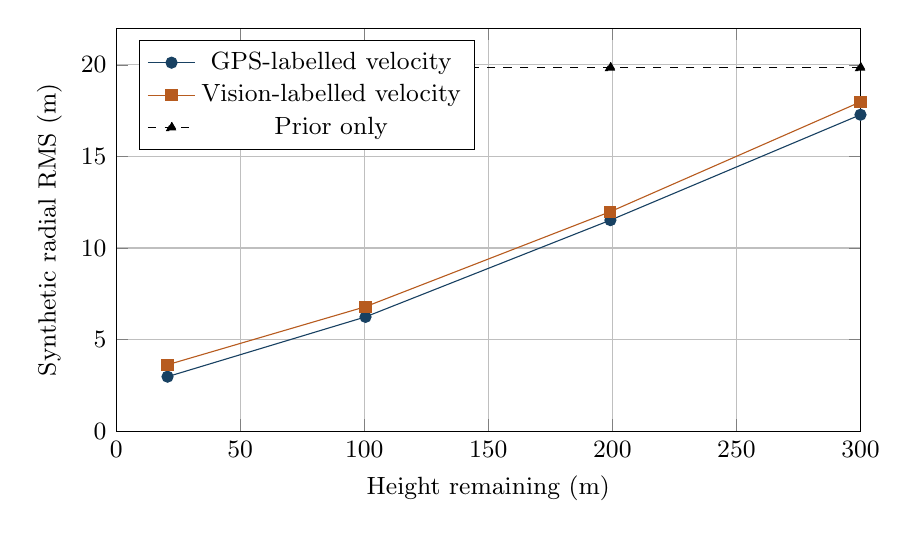
\begin{tikzpicture}
\begin{axis}[width=.91\linewidth,height=67mm,
 xlabel={Height remaining (m)},ylabel={Synthetic radial RMS (m)},
 xmin=0,xmax=300,ymin=0,ymax=22,grid=major,
 legend style={at={(.03,.97)},anchor=north west,font=\small},
 tick label style={font=\small},label style={font=\small}]
\addplot[color=atlasblue,mark=*] coordinates {(300.0000,17.276773) (199.2000,11.523467) (100.5000,6.242182) (20.7000,2.978762)};\addlegendentry{GPS-labelled velocity}
\addplot[color=atlasorange,mark=square*] coordinates {(300.0000,17.978586) (199.2000,11.987088) (100.5000,6.799342) (20.7000,3.629483)};\addlegendentry{Vision-labelled velocity}
\addplot[color=black,dashed,mark=triangle*] coordinates {(300.0000,19.837192) (199.2000,19.837192) (100.5000,19.837192) (20.7000,19.837192)};\addlegendentry{Prior only}
\end{axis}
\end{tikzpicture}
\end{center}
With no new information, the prior-only absolute endpoint covariance remains the same as height decreases. This is consistent with the fixed-endpoint theorem. Changing the remaining drift alone would answer a different covariance question.

\subsection{Averaging kernels reveal loss of independent information}
A separate piecewise-constant lag experiment on a 2.1 m grid between approximately 299 and 1 m uses the attached-eddy prior and $\ell=11.24$ m. It fixes the initial velocity perturbation to zero; it is a different boundary condition from the continuous-state descent Monte Carlo.
\begin{center}
\begin{tabular}{lrr}
\toprule
Noise model & DFS & Mean posterior SD (m/s)\\
\midrule
Independent GPS noise, 0.1 m/s & 43.12 & 0.226\\
Independent vision noise, 0.6 m/s & 14.98 & 0.402\\
Vision noise with known AR(1) correlation 0.85 & 12.52 & 0.572\\
\bottomrule
\end{tabular}
\end{center}
The correlated-noise row uses the full error covariance in the inverse. Correlation can sometimes improve particular high-frequency differences while reducing information in the mean or long-wave modes, so it is not a theorem that every correlation pattern reduces every DFS. These numbers apply to this chosen covariance and sampling grid.

\subsection{Deliberately mismatched sensor errors}
In a separate state-space experiment the true vision noise has the same marginal 0.6 m/s standard deviation but AR(1) correlation 0.85. The estimator incorrectly assumes independent noise. Near 100 m, coverage falls from 95.15\% to 81.6\%, and mean squared Mahalanobis distance rises from 2.003 to 3.499. Near 20.7 m, coverage is 50.65\%. The mean component layer RMS rises from 0.209 to 0.490 m/s.

The covariance underestimation is an outcome of a concrete misspecified model. It supports measuring temporal error covariance and incorporating it. Raising a protection multiplier after observing one test set is not a substitute for calibrating the underlying error model and evaluating fresh data.

\subsection{Verifying the remedy on exactly the same observations}
The added augmented-error filter uses the known $\rho=0.85$ and observation-error standard deviation 0.6 m/s. It is compared with the misspecified filter on the \emph{same} simulated trajectories and measurement realisations, not a new or easier dataset. The new error state has stationary prior variance $0.6^2$, and its innovation variance is $0.6^2(1-0.85^2)$. Its observation row adds that state to probe velocity, with no duplicate white observation variance.
\begin{center}
\begin{tabular}{rrrr}
\toprule
Height & Coverage: ignored & Coverage: tracked & Tracked mean $d^2$\\
(m) & (\%) & (\%) & \\
\midrule
300.0 & 94.75 & 94.75 & 1.978\\
199.2 & 91.35 & 95.20 & 2.006\\
100.5 & 81.60 & 94.85 & 2.015\\
20.7 & 50.65 & 95.10 & 1.998\\
\bottomrule
\end{tabular}
\end{center}
Near 100 m the corrected coverage is 94.85\%, versus 81.6\% when the correlation is ignored. Near 20.7 m it is 95.10\%, versus 50.65\%. The corrected predictor's RMS remains larger than the independent-noise baseline because the observations contain less information about persistent velocity offsets. Honest covariance restores calibration; it does not turn coloured errors into independent measurements.

The corrected mean component layer RMS is 0.428 m/s; its pointwise wind RMS is 0.587 m/s. These are synthetic results with the error correlation known exactly. Estimating correlation from a short flight and allowing uncertainty in it is additional work. The result shows that accounting for correlation can fix the particular demonstrated failure, rather than proving the model adequate for all sensor errors.

\subsection{Checking layer uncertainty rather than only layer accuracy}
For the 160--180 m layer, the synthetic grid contains nine samples. The posterior standard deviation is computed from \emph{all} smoother cross-height covariances. ``Diagonal SD'' wrongly treats those posterior errors as independent and is included to quantify the mistake. Coverage is the fraction of 4000 independent component realisations (two axes for each of 2000 drops) within the nominal two-sided 95\% interval.
\begin{center}
\begin{tabular}{lrrrr}
\toprule
Channel & Actual RMS & Posterior SD & Diagonal SD & Coverage\\
 & (m/s) & (m/s) & (m/s) & (\%)\\
\midrule
GPS, white & 0.060 & 0.059 & 0.066 & 94.65\\
Vision, white & 0.219 & 0.215 & 0.113 & 94.53\\
Coloured; ignored & 0.508 & 0.215 & 0.113 & 58.95\\
Coloured; tracked & 0.447 & 0.434 & 0.173 & 94.17\\
\bottomrule
\end{tabular}
\end{center}
For the independent vision channel, the covariance calculation gives 0.215 m/s, close to the observed 0.219 m/s RMS, whereas dropping cross terms gives 0.113 m/s. With correctly tracked coloured errors, the figures are 0.434, 0.447 and 0.173 m/s. The GPS-labelled diagonal-only calculation instead gives a \emph{larger} value than the correct covariance calculation. This confirms that the omitted terms do not have a universally positive sign.

The full corrected model's layer coverages range from approximately 94.2\% to 95.6\% over the eleven bins. Coverage estimates fluctuate, and the eleven estimates from the same descents are correlated. They must not be treated as eleven independent experiments. Correct means and uncertainties for continuous physical layers also require a verified quadrature/overlap definition, rather than simply relabelling a sample average.

\subsection{Release-velocity uncertainty: an independently simulated boundary test}
An additional dense inversion uses the same 2.1 m lag grid and wind kernel, independent white velocity noise 0.1 m/s, and a zero-mean perturbation model $u_0=0.7w_1+\eta_0$ with independent $\eta_0$ standard deviation 0.8 m/s. The joint prior's minimum covariance eigenvalue is positive, approximately 0.0111 in its stated units. Generate wind and release velocity by that constructive rule; then generate observations through the lag operator. Compare the wrongly fixed $u_0=0$ model with the correctly marginalised joint model.
\begin{center}
\begin{tabular}{lrrr}
\toprule
Release condition & First-sample RMS & Posterior SD & 95\% coverage\\
 & (m/s) & (m/s) & (\%)\\
\midrule
Incorrectly fixed & 1.813 & 0.198 & 17.27\\
Jointly estimated & 0.291 & 0.291 & 94.62\\
\bottomrule
\end{tabular}
\end{center}
The first wind cell is represented at its midpoint, 1.05 m below the initial height; its velocity observation is at the cell's lower boundary, after 2.1 m of descent. Treating an uncertain release velocity as known makes that observation look like direct wind information. The wrong posterior states an SD of 0.198 m/s while actual RMS is 1.813 m/s. Its interval coverage is only 17.275\%. Joint marginalisation gives posterior SD 0.291 m/s, RMS 0.291 m/s and coverage 94.625\%. This is an explicit boundary-condition counterexample to assuming an exact initial velocity for convenience.

The unknown initial condition has no arbitrary mean bias in this experiment; the failure is a missing uncertainty and correlation. Across all wind samples, RMS changes from 0.319 to 0.241 m/s. The numerical model is illustrative, rather than an estimate of ejection dynamics. The continuous-state descent Monte Carlo already uses a coupled random initial velocity; these dense inverse results are a separate test of how to handle that boundary in a gridded retrieval.

\subsection{Independent nonlinear dynamics test of the lag assumption}
The forward calculation here is not the linear estimator's own simulator. It integrates a vector-quadratic horizontal drag equation with fixed vertical relative speed 10.5 m/s, mean wind 5 m/s, and smooth gust $2\sin(0.7t)$ m/s for 20 s using RK4 at 1 ms. A lateral coefficient ratio $r$ multiplies the horizontal force without changing the prescribed vertical force balance. Wind is recovered from the exact simulated acceleration, with no measurement noise.
\begin{center}
\begin{tabular}{rrr}
\toprule
Lateral coefficient ratio $r$ & Using $\tau=v_d/g$ & Using calibrated $\tau=(v_d/g)/r$\\
 & Wind RMS (m/s) & Wind RMS (m/s)\\
\midrule
0.5 & 0.5700 & 0.0112\\
1.0 & 0.0042 & 0.0042\\
2.0 & 0.4929 & 0.0008\\
\bottomrule
\end{tabular}
\end{center}
The residual after calibration comes from retaining a linear inverse for nonlinear drag. A wrong lateral coefficient alone can consume the nominal 0.5 m/s wind budget even with perfect velocity and acceleration. These coefficient ratios are sensitivity cases, not measured canopy parameters.

State-space lag mismatch is also tested by halving or doubling the true lag while retaining the nominal estimator. Mean vision component layer RMS becomes 0.230 and 0.311 m/s, respectively. The difference from the nonlinear experiment is expected: smoothing, forcing spectrum, prior regularisation and the error metric differ. Neither test permits treating the nominal lag as measured.

\subsection{Numerical convergence and ground-layer sensitivity}
Midpoint-frozen coefficients are tested with one, two and four substeps per 5 Hz interval. At about 100 m the vision prediction's axis SD is 4.8040006, 4.8042459 and 4.8043083 m, respectively. Halving the substep reduces the change by about a factor of four, consistent with second-order coefficient freezing in this example. One-to-four-substep change is about 0.0064\%, which is small relative to the assumed model uncertainty.

At four substeps, varying the scale floor from 0.5 to 2 m changes that same axis SD by less than $6\times10^{-6}$ m. This small influence occurs in the chosen 100 m forecast and lag model; it is not a claim that touchdown conditions or all near-ground retrievals are insensitive to boundary-layer physics. The example profiles and full sensitivity outputs are preserved, with their simulation labels.

\section{Coverage, unresolved questions, and engineering handoff}
\label{sec:handoff}
\subsection{Coverage of the proposal's mathematical index}
This table traces every topic in Appendix E. ``Derived'' means established with the stated hypotheses in this document, rather than experimentally validated. Stretch techniques are included mathematically even though they need not be flown.
\begin{longtable}{p{0.60\linewidth}p{0.28\linewidth}}
\toprule
Topic & Derivation location\\
\midrule
\endfirsthead
\toprule Topic & Derivation location\\\midrule\endhead
Pinhole camera; ground-plane homography & Navigation section\\
FFT NCC; sub-pixel peak; covariance; RANSAC & Navigation section\\
Terminal velocity; canopy sizing; hypsometric altitude & Physics section\\
Horizontal lag and inversion conditioning & Physics and retrieval sections\\
Pendulum specific force; forcing spectrum & Physics section\\
Error-state EKF; quaternion attitude; reset; reprojection derivatives & Navigation section\\
Innovation gating; NEES; information bound; protection level & Navigation section\\
Tilt--translation separation; timing; error budget; crossover & Navigation section\\
Shear path and frozen-field approximation & Physics section\\
Drop-Dryden transverse covariance; scale deformation; exact states & Section~\ref{sec:turbulence}\\
Kalman filtering; smoothing; Gaussian-process inverse & Section~\ref{sec:retrieval}\\
Averaging kernels; degrees of freedom; layer covariance & Section~\ref{sec:retrieval}\\
Landing position and time; Mahalanobis calibration & Section~\ref{sec:landing}\\
Marginal likelihood; model-comparison limitations & Section~\ref{sec:retrieval}\\
Potential temperature; MOST; Richardson number; roughness fit & Boundary-layer section\\
Pendulum response as a shear/turbulence diagnostic & Physics section\\
Landing uncertainty shrinkage & Section~\ref{sec:landing}: fixed-endpoint theorem; moving-drift counterexamples\\
Map-datum gauge; survey uncertainty & Navigation section\\
Truncated least squares; lifted QCQP and SDP certificate conditions & Navigation section\\
Submodular landmark selection and its normalised guarantee & Navigation section\\
Uncertainty-aware notional target selection & Navigation section\\
Footprint, blur, sample count, storage, compute, power, loads and radio & Engineering section\\
\bottomrule
\end{longtable}

\subsection{Completed and strongest evidence}
The proposal's mathematics has been assembled into a coherent reference with a consistent camera convention, stated physical assumptions, explicit derivations, corrected probability claims, and worked examples. The exact turbulence realisation, covariance positivity, descent time conversion, inverse lag, Gaussian conditioning, smoothing, and fixed-endpoint monotonicity have analytic derivations. The numerical suite verifies independent formulations and limiting cases, with retained synthetic outputs.

The strongest simulation result is conditional: matched known parameters yield well-calibrated landing ellipses and sub-0.5 m/s layer errors in the synthetic case. The strongest engineering caution is also quantified: unmodelled error correlation severely reduces coverage, and uncalibrated lateral response can produce order-0.5 m/s wind bias despite perfect motion measurements.

The built-in editor's compilation was attempted and failed before producing a PDF with the environment message ``Unable to find standard directories for platform.'' Source brace/environment checks, unique-label checks and reference checks are separate from compilation. No rendered page layout, line overflow or package availability has been verified. The saved standalone source is preserved for the editor or another LaTeX installation; no compiler or plugin was installed.

\subsection{Decisions and assumptions}
The original proposal and the original numerical examples have been preserved as source material. This document records corrections without adopting a new mission architecture or declaring a physically unmeasured model to be true. Hardware selection has since advanced: the current BOM/platform summary is in \texttt{design\_baseline.md}. Numerical camera footprint, blur, image-storage and processing examples using $1280\times800$, $90^\circ$ horizontal field of view, or historical Orange Pi H618/OV9281 assumptions remain illustrative calculations only. They are not estimates of current IMX296 image geometry, Pi Zero 2 W throughput, or flight performance. Recompute those quantities only from calibrated camera intrinsics/optics and measured target-hardware timing. No large dependency, external service, flight rule or canopy design has been introduced. The numerical model uses NumPy, known Gaussian parameters, a stated near-ground scale floor, two independent horizontal axes, and labelled synthetic velocity channels. Certifiable registration is described with its necessary primal-feasibility and optimality conditions; no actual SDP flight fix or numerical global-optimality certificate is claimed.

\subsection{What still requires measurements or project decisions}
\begin{enumerate}
\item \textbf{Canopy dynamics.} Measure terminal speed, lateral response, deployment transient and pendulum motion. Fit $\tau_h$ or a lateral drag model with confidence intervals. A vertical descent-rate measurement alone does not select the horizontal model.
\item \textbf{Camera and inertial calibration.} Determine intrinsics, distortion, extrinsics, lever arms, exposure timing and timestamp uncertainty. Test map matches over representative terrain; measure failures, first-fix time, bias and temporal covariance.
\item \textbf{Truth quality.} Survey map control points with quantified uncertainty, and log independent position/velocity truth. GPS alone does not supply all fifteen navigation error-state components for a full-state NEES calculation.
\item \textbf{Atmospheric inference.} Measure thermistor response in flight-like airflow, pressure/density uncertainties, mast representativeness and relevant stability flux information or jointly identifiable MOST profiles. Assess displacement height and heterogeneous fetch before reporting roughness.
\item \textbf{Retrieval independence.} Quantify the shared attitude, lag and prior errors in image-versus-GPS wind comparisons. A common bias can cancel in their difference.
\item \textbf{Calibration across drops.} Evaluate prediction ellipses and time intervals on independent descents, with predeclared metrics and model tuning separate from validation. A single flight cannot test 95\% long-run landing coverage.
\item \textbf{Stretch certification.} Select the exact registration relaxation, bounds and solver tolerances before issuing an SDP certificate; rank appearance alone is insufficient. Safe-target reachability is hypothetical for a passive canopy.
\item \textbf{Requirements.} Confirm the current competition rules, actual radio configuration, mass convention, load cases, battery and processing budgets before asserting compliance.
\end{enumerate}

\subsection{Highest-value next action}
First establish the current BOM hardware configuration, then conduct a short, time-synchronised suspension/drop calibration using the selected IMX296 camera, BMI088 IMU, MS5611 pressure sensor and independent velocity truth. Use it first to estimate canopy lateral response and sensor-error correlation, then rerun the same mathematical model with those measured uncertainties. This directly tests the two assumptions that dominate the demonstrated gap between an internally consistent simulation and a reliable wind/landing result. Preserve raw logs and calibration metadata so later navigation and atmosphere analysis can be repeated.

\subsection{Reference provenance}
The local secondary mission proposal is \texttt{wiki/trn\_secondary\_mission\_proposal.md}, draft 27 September 2026. The current hardware reference is \texttt{wiki/design\_baseline.md}; older proposal and simulation parameters are retained with their stated historical scope. Primary literature, manufacturer formulas and theorem sources are linked beside the relevant derivations. Derivations shown here are worked calculations for this project, not copied passages from those sources.

The connected reference folder is \url{https://drive.google.com/drive/folders/1ugYnjOalW-hIZqXO9nSJtGS6KleoJ3KW}. Its listed Control Systems and Design Reviews folders were empty when inspected. The fetched historical regulations were \url{https://drive.google.com/file/d/1LubKeC729i9NbmgHwG-wzu4gwhDO1PfJ/view}. No Drive document was edited. No recent Git history was available because this local folder was not a Git checkout.
\end{document}
